\documentclass[UTF8]{article}


\usepackage{arxiv}
\usepackage{ctex}
\usepackage[utf8]{inputenc} % allow utf-8 input
\usepackage[T1]{fontenc}    % use 8-bit T1 fonts
\usepackage{hyperref}       % hyperlinks
\usepackage{url}            % simple URL typesetting
\usepackage{booktabs}       % professional-quality tables
\usepackage{amsfonts}       % blackboard math symbols
\usepackage{nicefrac}       % compact symbols for 1/2, etc.
\usepackage{microtype}      % microtypography
\usepackage{lipsum}
\usepackage{indentfirst}
\usepackage{graphicx}
\usepackage{float}
\usepackage{caption}
\usepackage{subfigure}
\setlength{\parindent}{2em}
\usepackage{listings}
\usepackage{algorithm}  
\usepackage{algpseudocode}  
\usepackage{amsmath}


\setlength{\parindent}{2em} 
\title{Information Retrieval Course Project \\
	Kok-Kip Search Engine}



\author{
	\textbf{Liang Yucheng} \\
	\textbf{16340133} \\
	School of Data and Computer Science\\
	Sun Yat-sen University\\
	Guangzhou, Guangdong, China 510006 \\
	\textbf{jacky14.liang@gmail.com} \\
	\and
	\textbf{Liang Junhua} \\
	\textbf{16340129} \\
	School of Data and Computer Science\\
	Sun Yat-sen University\\
	Guangzhou, Guangdong, China 510006 \\
	\textbf{alva112358@gmail.com} \\
	\and
	\textbf{Zeng Guangtao} \\
	\textbf{16340010} \\
	School of Data and Computer Science\\
	Sun Yat-sen University\\
	Guangzhou, Guangdong, China 510006 \\
	\textbf{kids937@foxmail.com} \\
}

\begin{document}
	\maketitle
	
	% Abstract
	\begin{abstract}
		Search Engine is an indispensable part of people's daily life and document searching is an important branch of the field of information retrieval. What we have achieved in this project is a document-oriented serach engine, which is supposed to deliver great search results to users. The most creative part in our project is our score system, which is facilited by the ensemble idea that bagging various scores to rank documents reasonably based on their semantic similarities toward query words. Even if this is a small course project, under align development, we still have a frontend and a backend seperately, providing premium searching experience for users.
	\end{abstract}
	
	
	% keywords
	\keywords{Information Retrieval \and Search Engine \and Document Retrieval \and Word Embedding}
	
	
	% github link
	Github Link: https://github.com/Kok-Kip
	
	
	% Part 1: Introduction.
	\section{Introduction}
	In the last ten years, search engine has become a useful tool for people. People search nearly everything with an serach engine, including papers, news, documents, government websites and so on. Now we have a variety of advanced search engines, such as Bing, Google, Search Encrypt, Yandex, Swisscows. Considering that Information Retrieval Course mainly focuses on document retrieval, we are looking forward to implementing a creative document-oriented search engine by applying some of the methods covered in class. We have traditional methods like tf-idf and bm25, mainly considering the document relevance regarding query words. Also we make full use of the latest technology, word embedding. With word embedding, we are able to discover the semantic similarty between words and documents, which is difficult to be captured by traditional methods.
	
	This paper will be illustrated in the following ways: In Section 2, some related works will be discussed, some of which have inspired this project more or less. And I will uncover the details behind this engine in Section 3, both principles and applications. In Section 4, we will present the result of our search engine. And in the last section, we may sumarize our project and describe some future works.
	
	
	
	
	% Part 2: Related Works.
	\section{Related Works}
	Nowadays, there are a great number of search engines that feed different kinds of users. Google is a popular search engine that performs well in nearly all kinds of searching. And Google Scholar is a document search system that contains millions of papers. PageRank facilitate Google in ranking valuable and popluar pages by considering their linking relationships in network. Bing performs better than other rivals in image searching across all browsers, while Search Encrypt focuses on information privacy by encrpting queries. And Yandex is the most popular search engine in Russia, offering a suite of pretty cool tools. So there are variour kinds of search engine and our project only concentrate on document searching.
	
	In terms of document retrieval, in SimSeerX, Kyle Williams presents a content-based document retrieval engine to allow a document-to-document query. There are three major algorigthm: Key Phrase Similarity, Shingle Similarity and Simhash Similarty. Key Phrase Similarity is mainly based on BM25, extracting key words from a formatted document. Shingle Similarty is inspired by k-gram algorithm. It first generates a serious of shinglings and then hashes words to number in order to calculate similarity. Simhash Similarity maps a document into a 64-bits vector and then use the hamming distance to determine the similarity between two documents. 
	
	Most of the methods mentioned above prefer to compress a document into a high dimension vector, which may cause a considerable information loss and thus lead to a huge amount computation. Therefore, we put our effor to use new advanced methods to optimize query result, like word embedding. Our ultimate aim is to deliver good quality result in a short time.
	
	
	% Part 3: Design and Alogrithm
	\section{Design and Algorithm}
	As our search engine mainly focuses on document retrieval, we concentrate on developing a score system to deliver good result to users. Our score system combines three algorithms: tf-idf, bm25 and word embedding. The simple reason why we choose these methods is that they complement each other. While tf-idf and bm25 prefer exact matching and valuable words, word embedding favors related words based on semantic similarity. Inspired by the idea of model bagging, we assign different weight to these algorithms and add them linearly. By doing so, we can both capture those key words and return the most relevant document. Also we have other tricks to improve the quality and efficiency of searching. In the following passage we are going to elaborate the details of implementation.
	
	
	% Part 3.1: Dataset
	\subsection{Document Dataset}
	All documents are download from a chinese news website. The size of our dataset is about 100 and we may enlarge it in the future if we have enough compuatational resource.
	
	
	% Part 3.2: Database
	\subsection{Database Design}
	Database storage is of utmost significance for a search engine. A well-designed storage structure may benefit search efficiency. We prefer construct our database offline in order to speed up query time. We store words, documents and their relationship seperately in three tables. Also, out of consideration for computation, we store word embedding for each word in database as bytes, we can significantly reduce calculating time when a query is requested.
   Because database model is not the main point of this report, you can gain more details in Github, where we place our design doc.
	
	% Part 3.3: Algorithm
	\subsection{Algorithm}
	Currently we have ensembled three different algorithms to calculate score.
	
	% Part 3.3.1: TF-IDF
	\subsubsection{TF-IDF}
	In the information retrieval system, we first adopt TF-IDF(Term Frequency Inverse Document Frequency) algorithm to calculate the word relevance in document queries. It's a really popular algorithm  [In the information retrieval system, we first adopt TF-IDF algorithm to calculate.md](In the information retrieval system, we first adopt TF-IDF algorithm to calculate.md) which has been used by most online search engines.The algorithm weighs a term's frequency in a document and calculate its inverse document frequency through all the documents. The product of the TF and IDF of the term is the final score for the document in a query.
	
	For a term $t$ and a document $d$, the weight(score) $W_{t,d}$ is given by:
	\[ W_{t,d} = TF_{t,d}log[N/DFT] \]
	Where $TF_{t,d}$ is the number of occurrences of $t$ in document $d$, $DFT$ is the number of documents that involve the term $t$, and $N$ is the total document number.
	
	In the system, we get the query, remove the empty words, throw in the function and then we can get the relevant scores of all the documents, which make us efficient to get the most favorite document in the query.
	
	% Part 3.3.2: BM25
	\subsubsection{BM25}
	To improve the performance of the system, we also apply BM25 algorithm to make up the TF-IDF. Although BM25 is based on TF-IDF, it comes from probabilistic information retrieval in which relevance score can reflect the probability a user will consider the result relevant. Compared with TF-IDF, BM25 use document length to make the score more accurate. Here the formula is given by:
	\[ W_{t,d} = \frac{f_t (k_1+1)}{f_t+K}
	\\ K = k_1(1 - b + b \times \frac{dl}{avgdl}) \]
	Where $k_1$ and $b$ are regulatory factors (generally $k_1 = 2$, $b=0.75$). In addition, dl is the length of the document.
	
	It can be shown in the definition of K, the factor $b$ decides how the length of the document can affect the score. The bigger $b$ gets, the more influence the length make on the relevance. Due to such a wonderful feature, we import BM25 to make the system work better.
	
	% Part 3.3.3: Word Embedding
	\subsubsection{Word Embedding}
	In this project, we use the most popular word embedding model -- word2Vec model. It can be obtained using two methods: Skip Gram and Common Bag Of Words(CBOW). The input is the one-hot encoding of a word and the output is the probability of the occurance of other words. The higher probability between two words, the closer they stay in the semantic space.
	
	\begin{figure}[H]
		\centering
		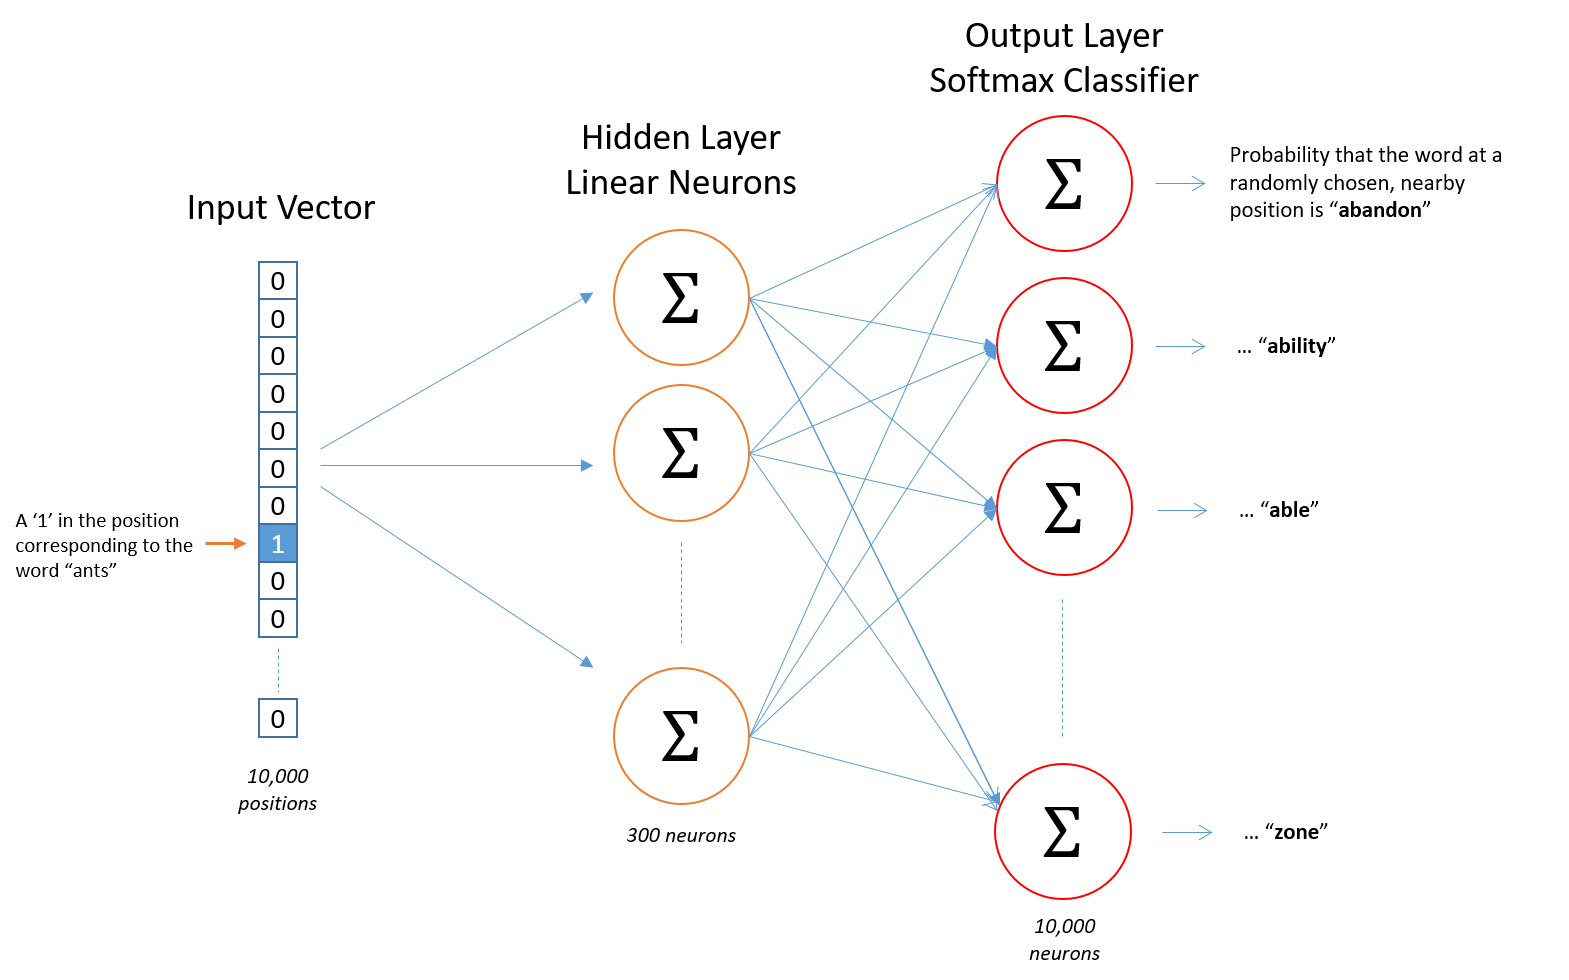
\includegraphics[width=0.7\linewidth]{./image/img16}
		\caption{The process of skip-gram model. Source: \url{https://www.cnblogs.com/micrari/p/9115426.html}}
		\label{fig:img1}
	\end{figure}
%\href{https://www.cnblogs.com/micrari/p/9115426.html}
	
	Gensim can compute the similarity score between two embedding vectors easily, but it is mostly based on Euclidean Distance, which may unreliable when two vectors have different in length. Instead, we use cosine similarity and it is proven reliable even two vectors have different length.
	
	Undoubtedly it is time-consuming and extremely difficult to train a good model by us own in such short time. Luckily, with the help of Tencent AI Lab Embedding Corpus for Chinese Words and Phrases, we are able to construct a word2Vec model easily in Python. However for a real time search engine, it still takes long time to load from the dataset, so we decide just use a portion of it. By doing experienments repeatly, we make a trade-off between accuracy and efficency. And finally we use 700,000 records out of 8, 000, 000 in the dataset, which still deliver good search results.
	
	
	% Part 4: Experiment Result
	\section{Result}
	We evaluate our product from vairous angles. Firstly, we care about the latency of a query. Here we use end-to-end time to evaluate the speed of a query. Second, we expect a good result but it is difficult to quantify. Questionnaire is a good alternative but we don't have many users. So instead we merely evaluate the result based on our feeling. 
	
	% Part 4.1: MainPage
	\subsection{Search Engine MainPage}
	We have implemented a beautiful website to present our results. Some snapshots are diplayed as follows.

	\begin{figure}[H]
		\centering
		\subfigure{
			\begin{minipage}[]{0.5\linewidth}
				\centering
				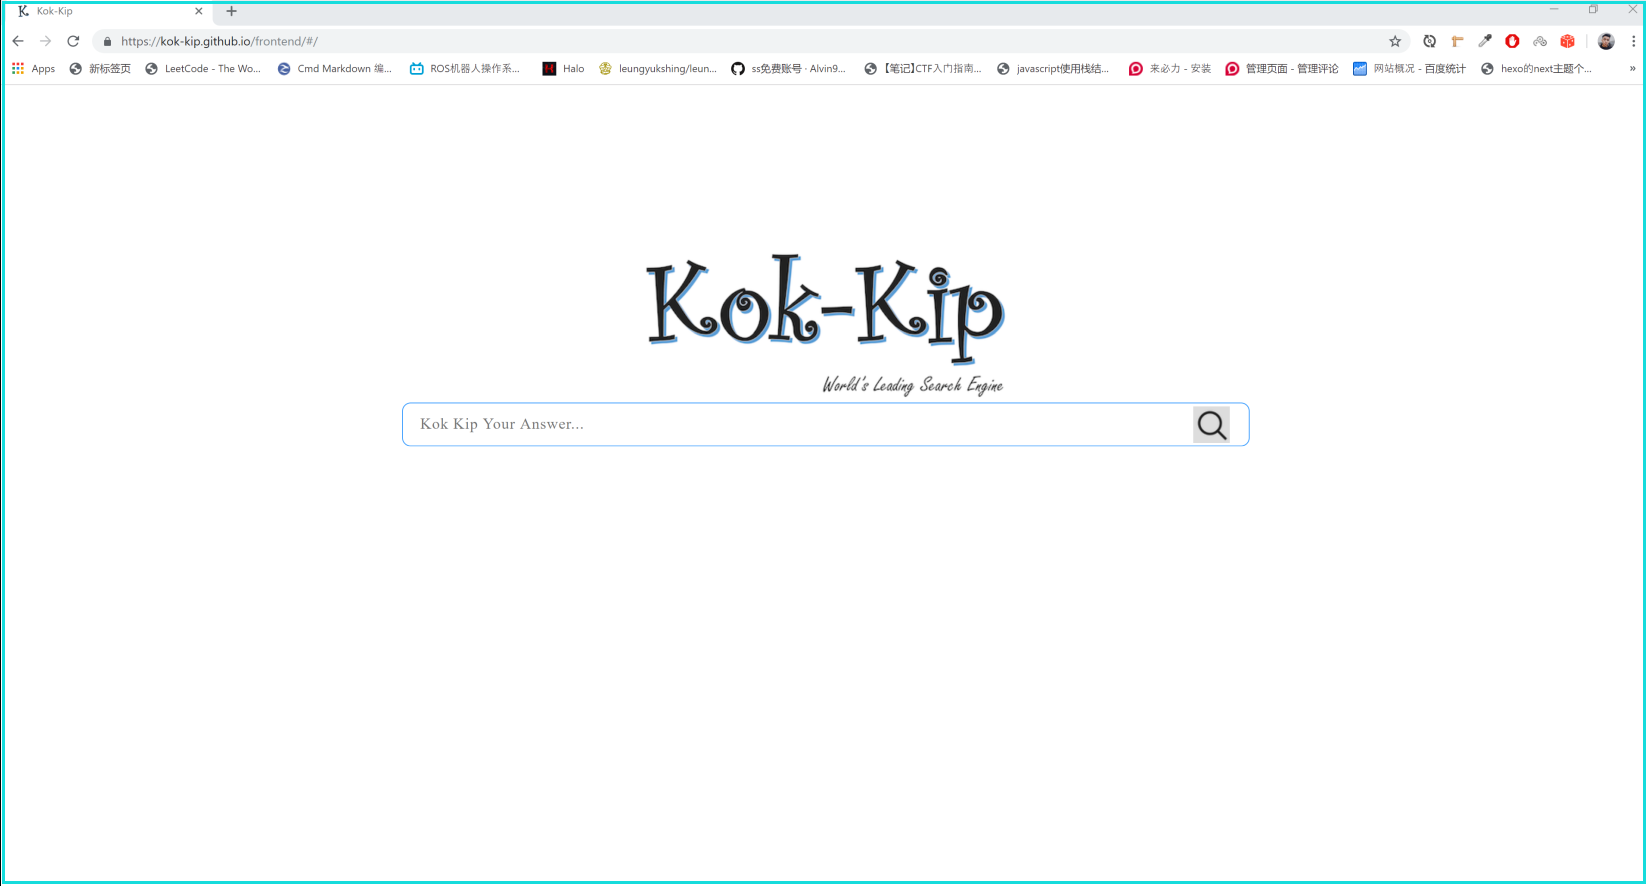
\includegraphics[width=3in]{./image/img1}
				\caption{MainPage}
			\end{minipage}%
		}%
		\subfigure{
			\begin{minipage}[]{0.5\linewidth}
				\centering
				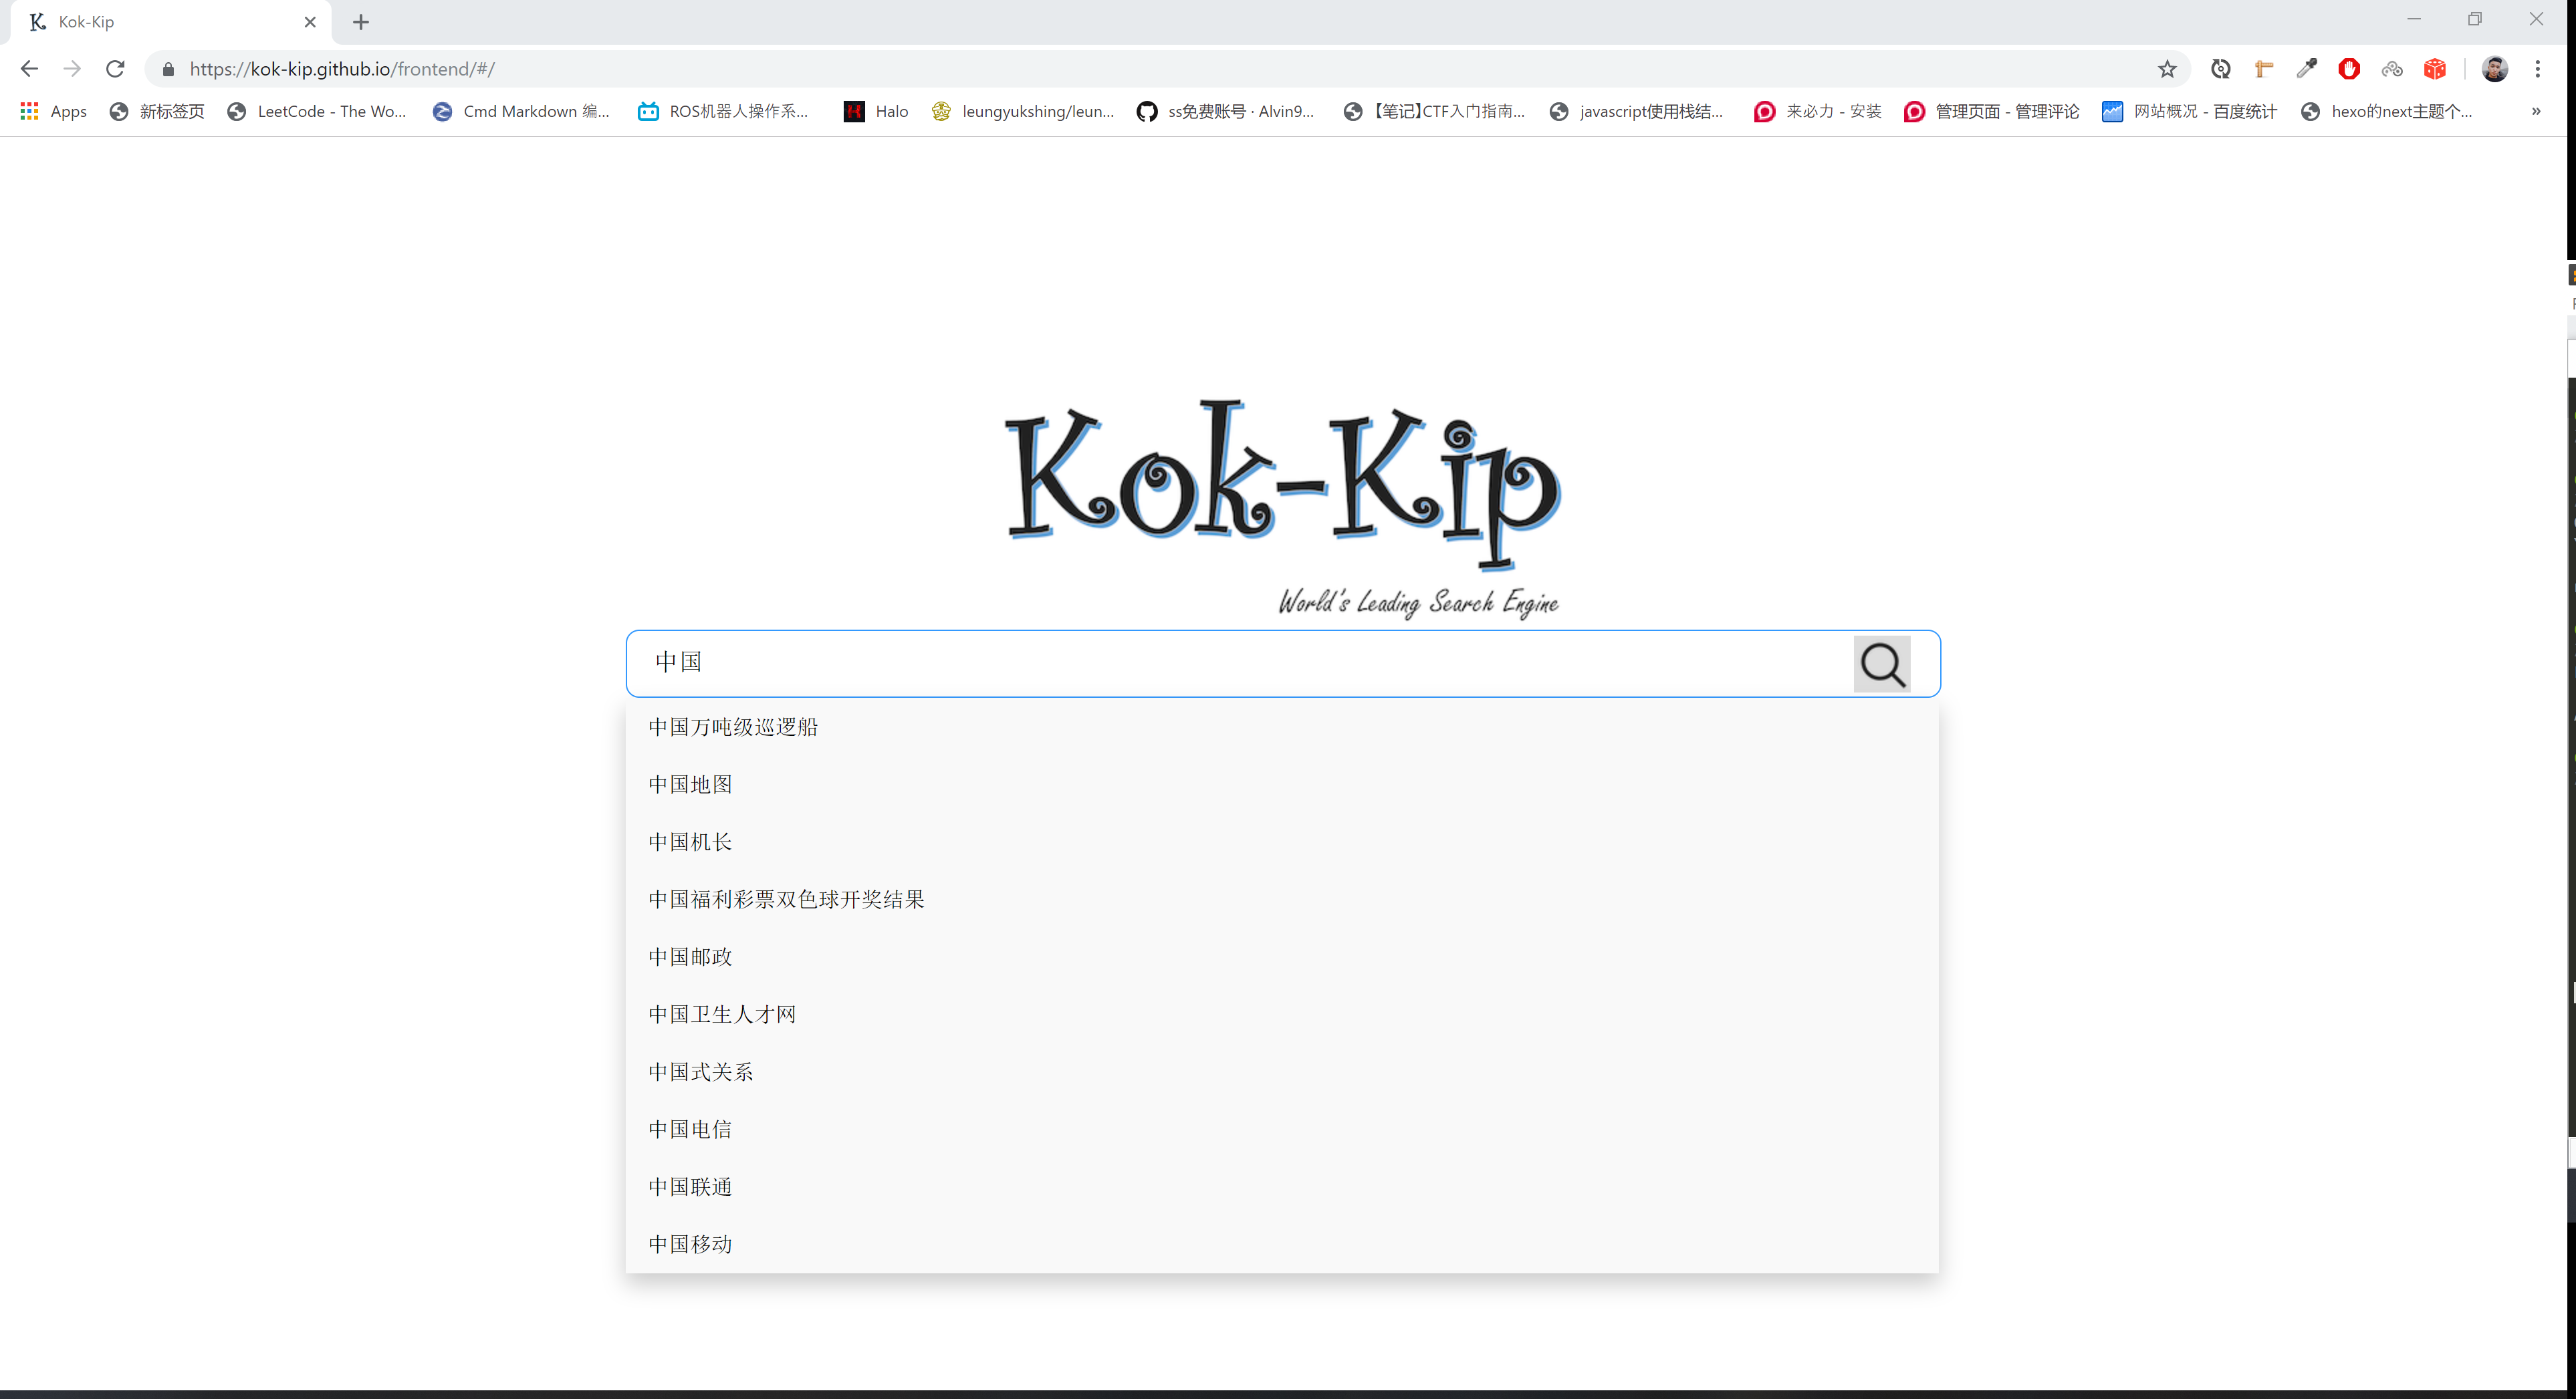
\includegraphics[width=3in]{./image/img2}
				\caption{Search Suggestions}
			\end{minipage}%
		}%
		\centering
	\end{figure}
	
	% Part 4.2: Search Result
	\subsection{Search Result}

	% Part 4.2.1: Query 1
	\subsubsection{Query Word: 细胞}
	\begin{figure}[H]
		\centering
		\subfigure{
			\begin{minipage}[]{0.5\linewidth}
				\centering
				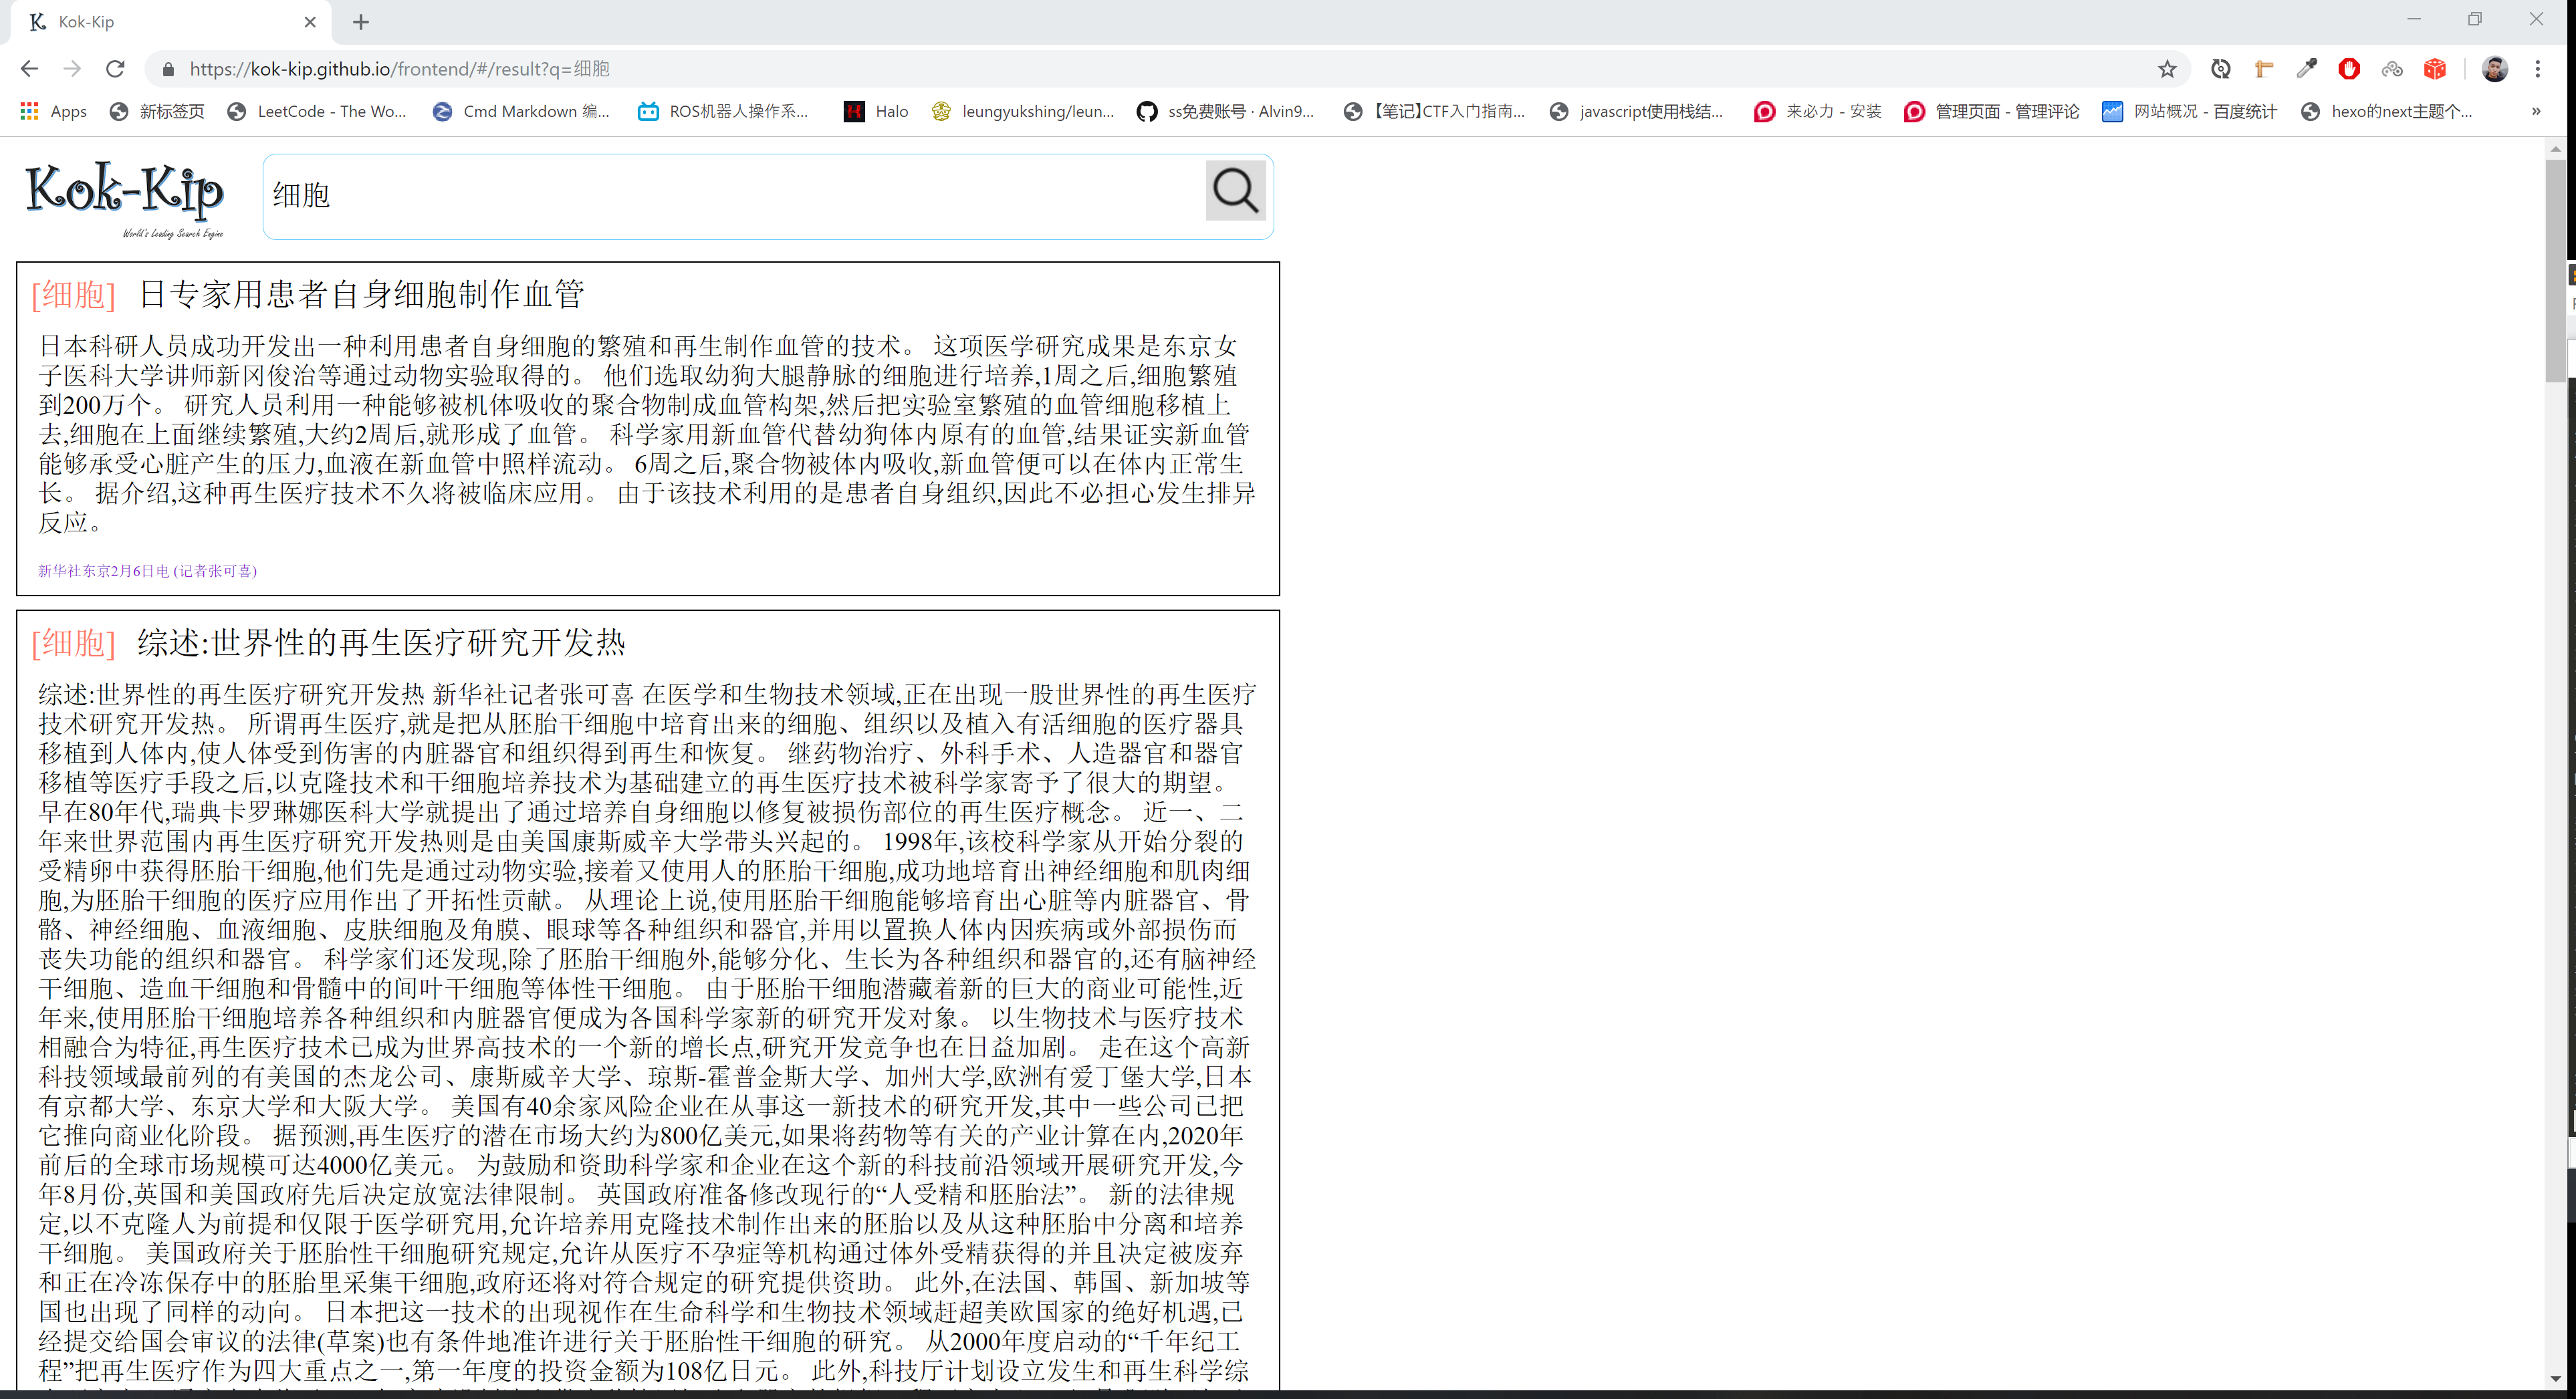
\includegraphics[width=3in]{./image/img3}
				\caption{Search Result for 细胞 1}
			\end{minipage}%
		}%
		\subfigure{
			\begin{minipage}[]{0.5\linewidth}
				\centering
				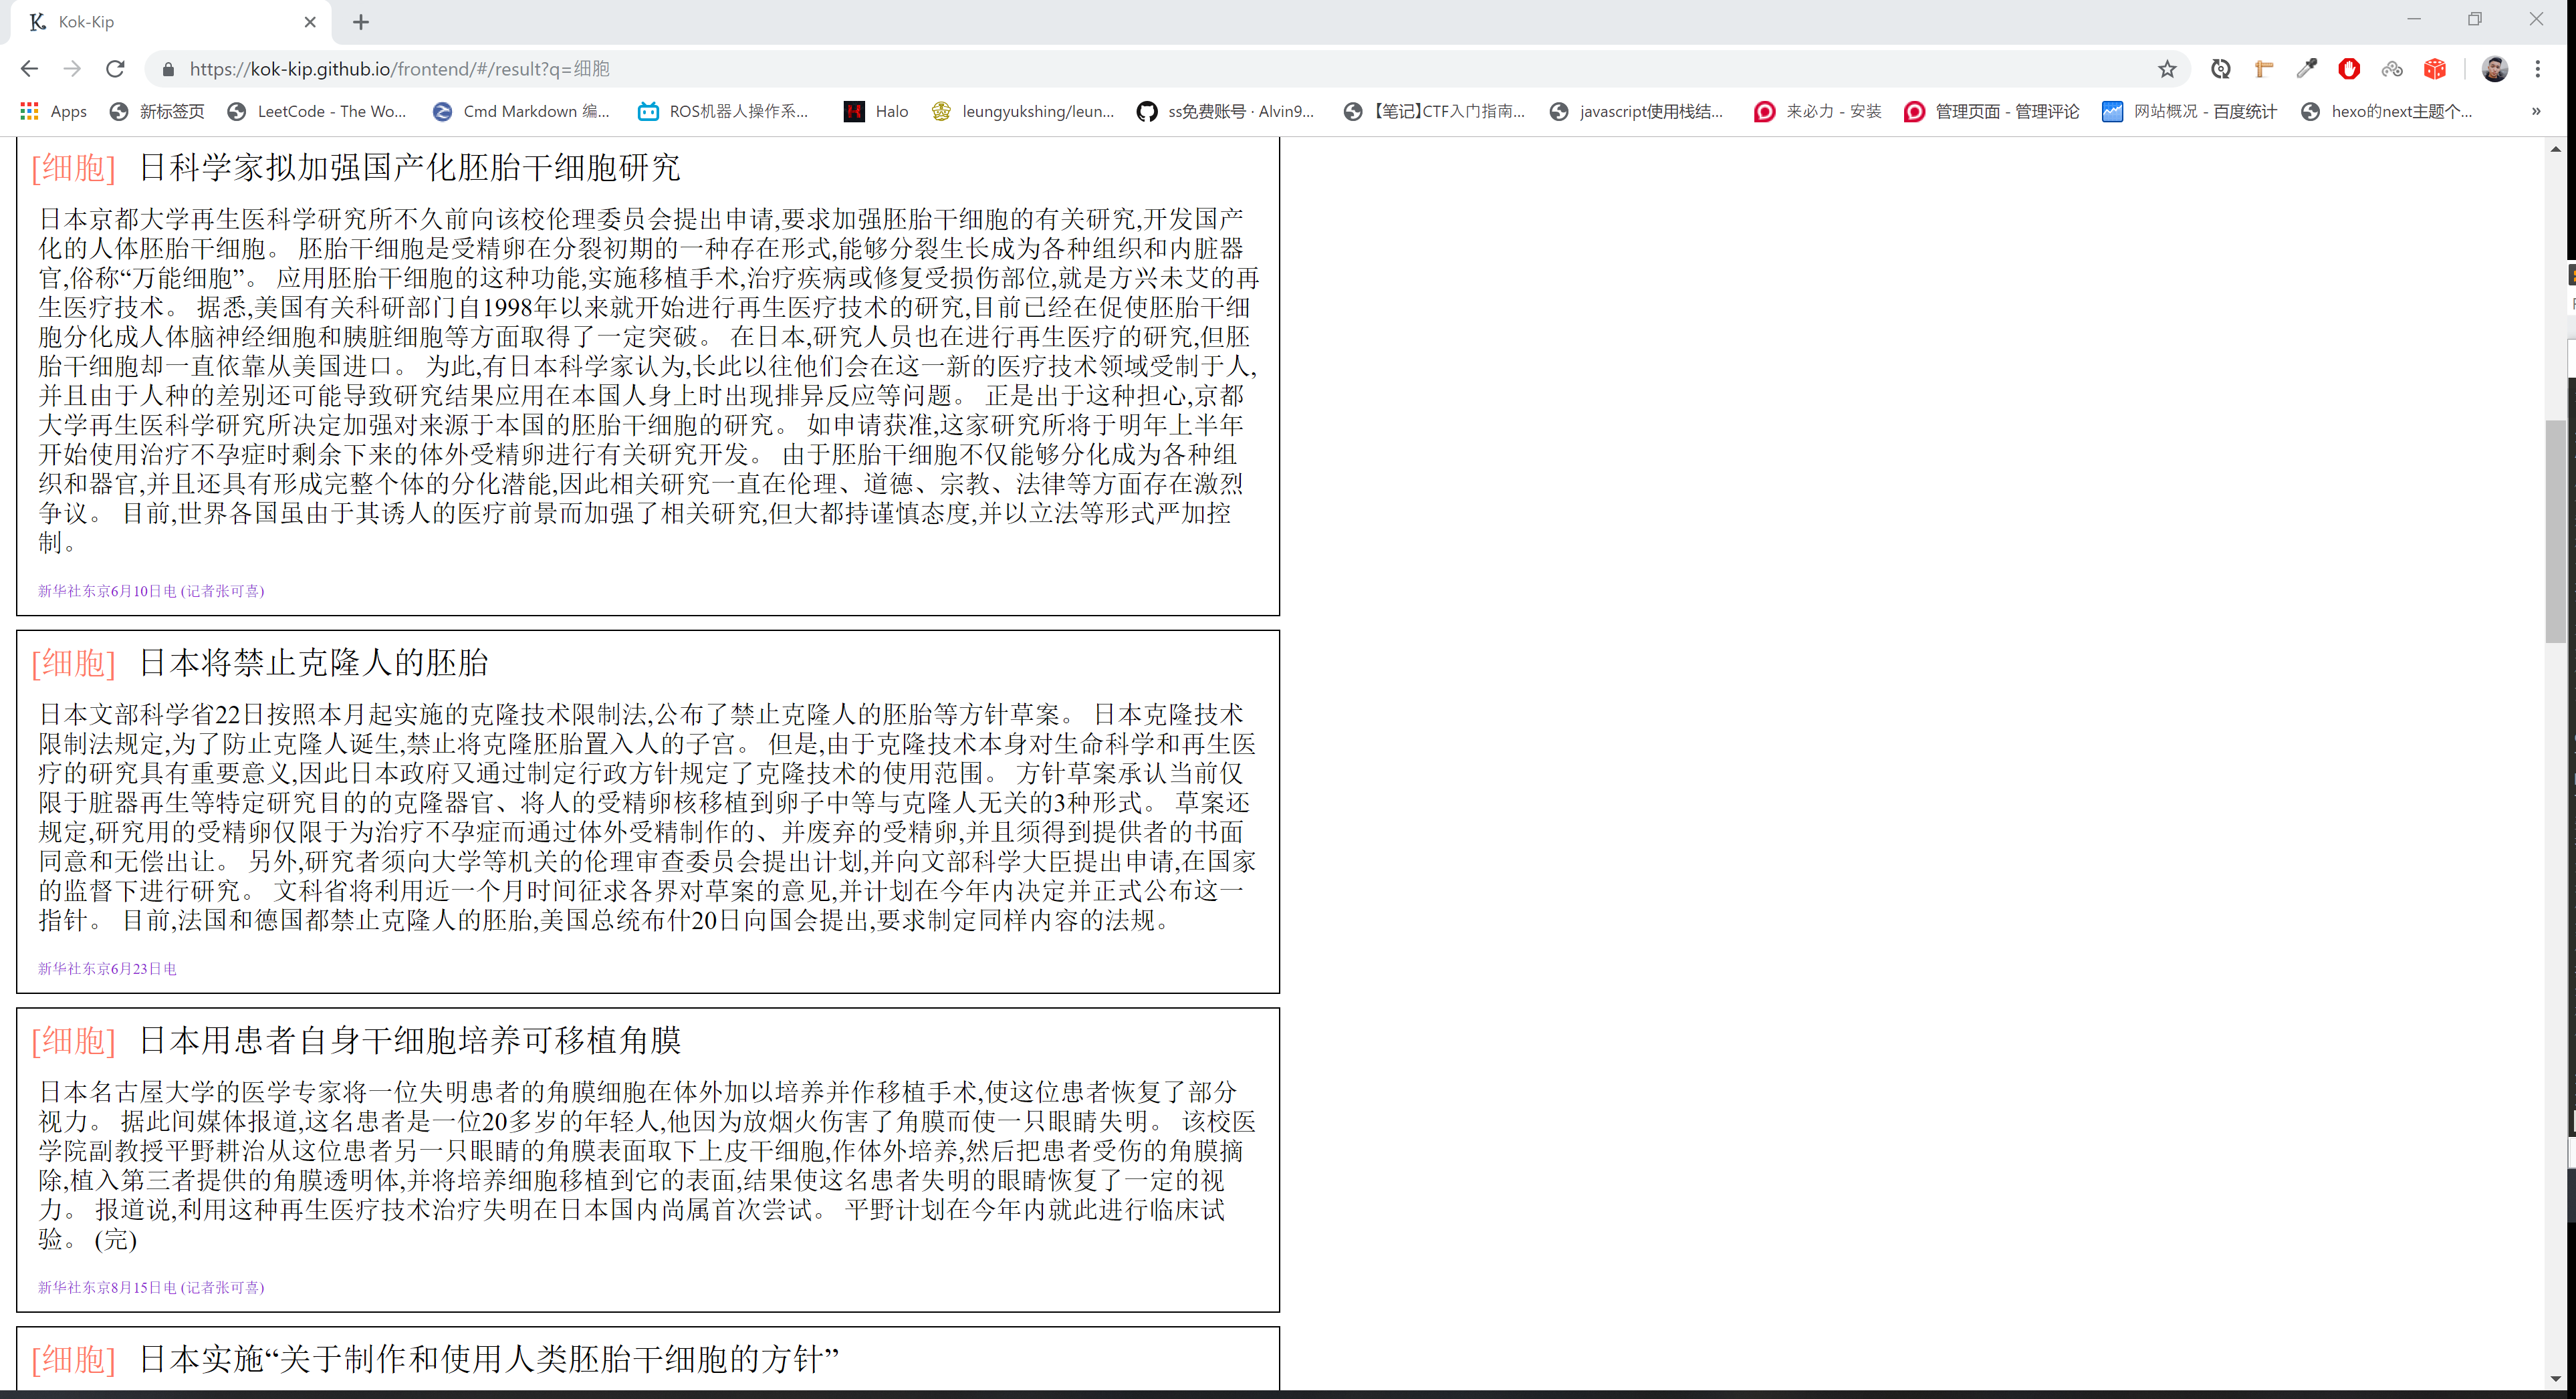
\includegraphics[width=3in]{./image/img4}
				\caption{Search Result for 细胞 2}
			\end{minipage}%
		}%
		\centering
	\end{figure}
	
	\begin{figure}[H]
		\centering
		\subfigure{
			\begin{minipage}[]{0.5\linewidth}
				\centering
				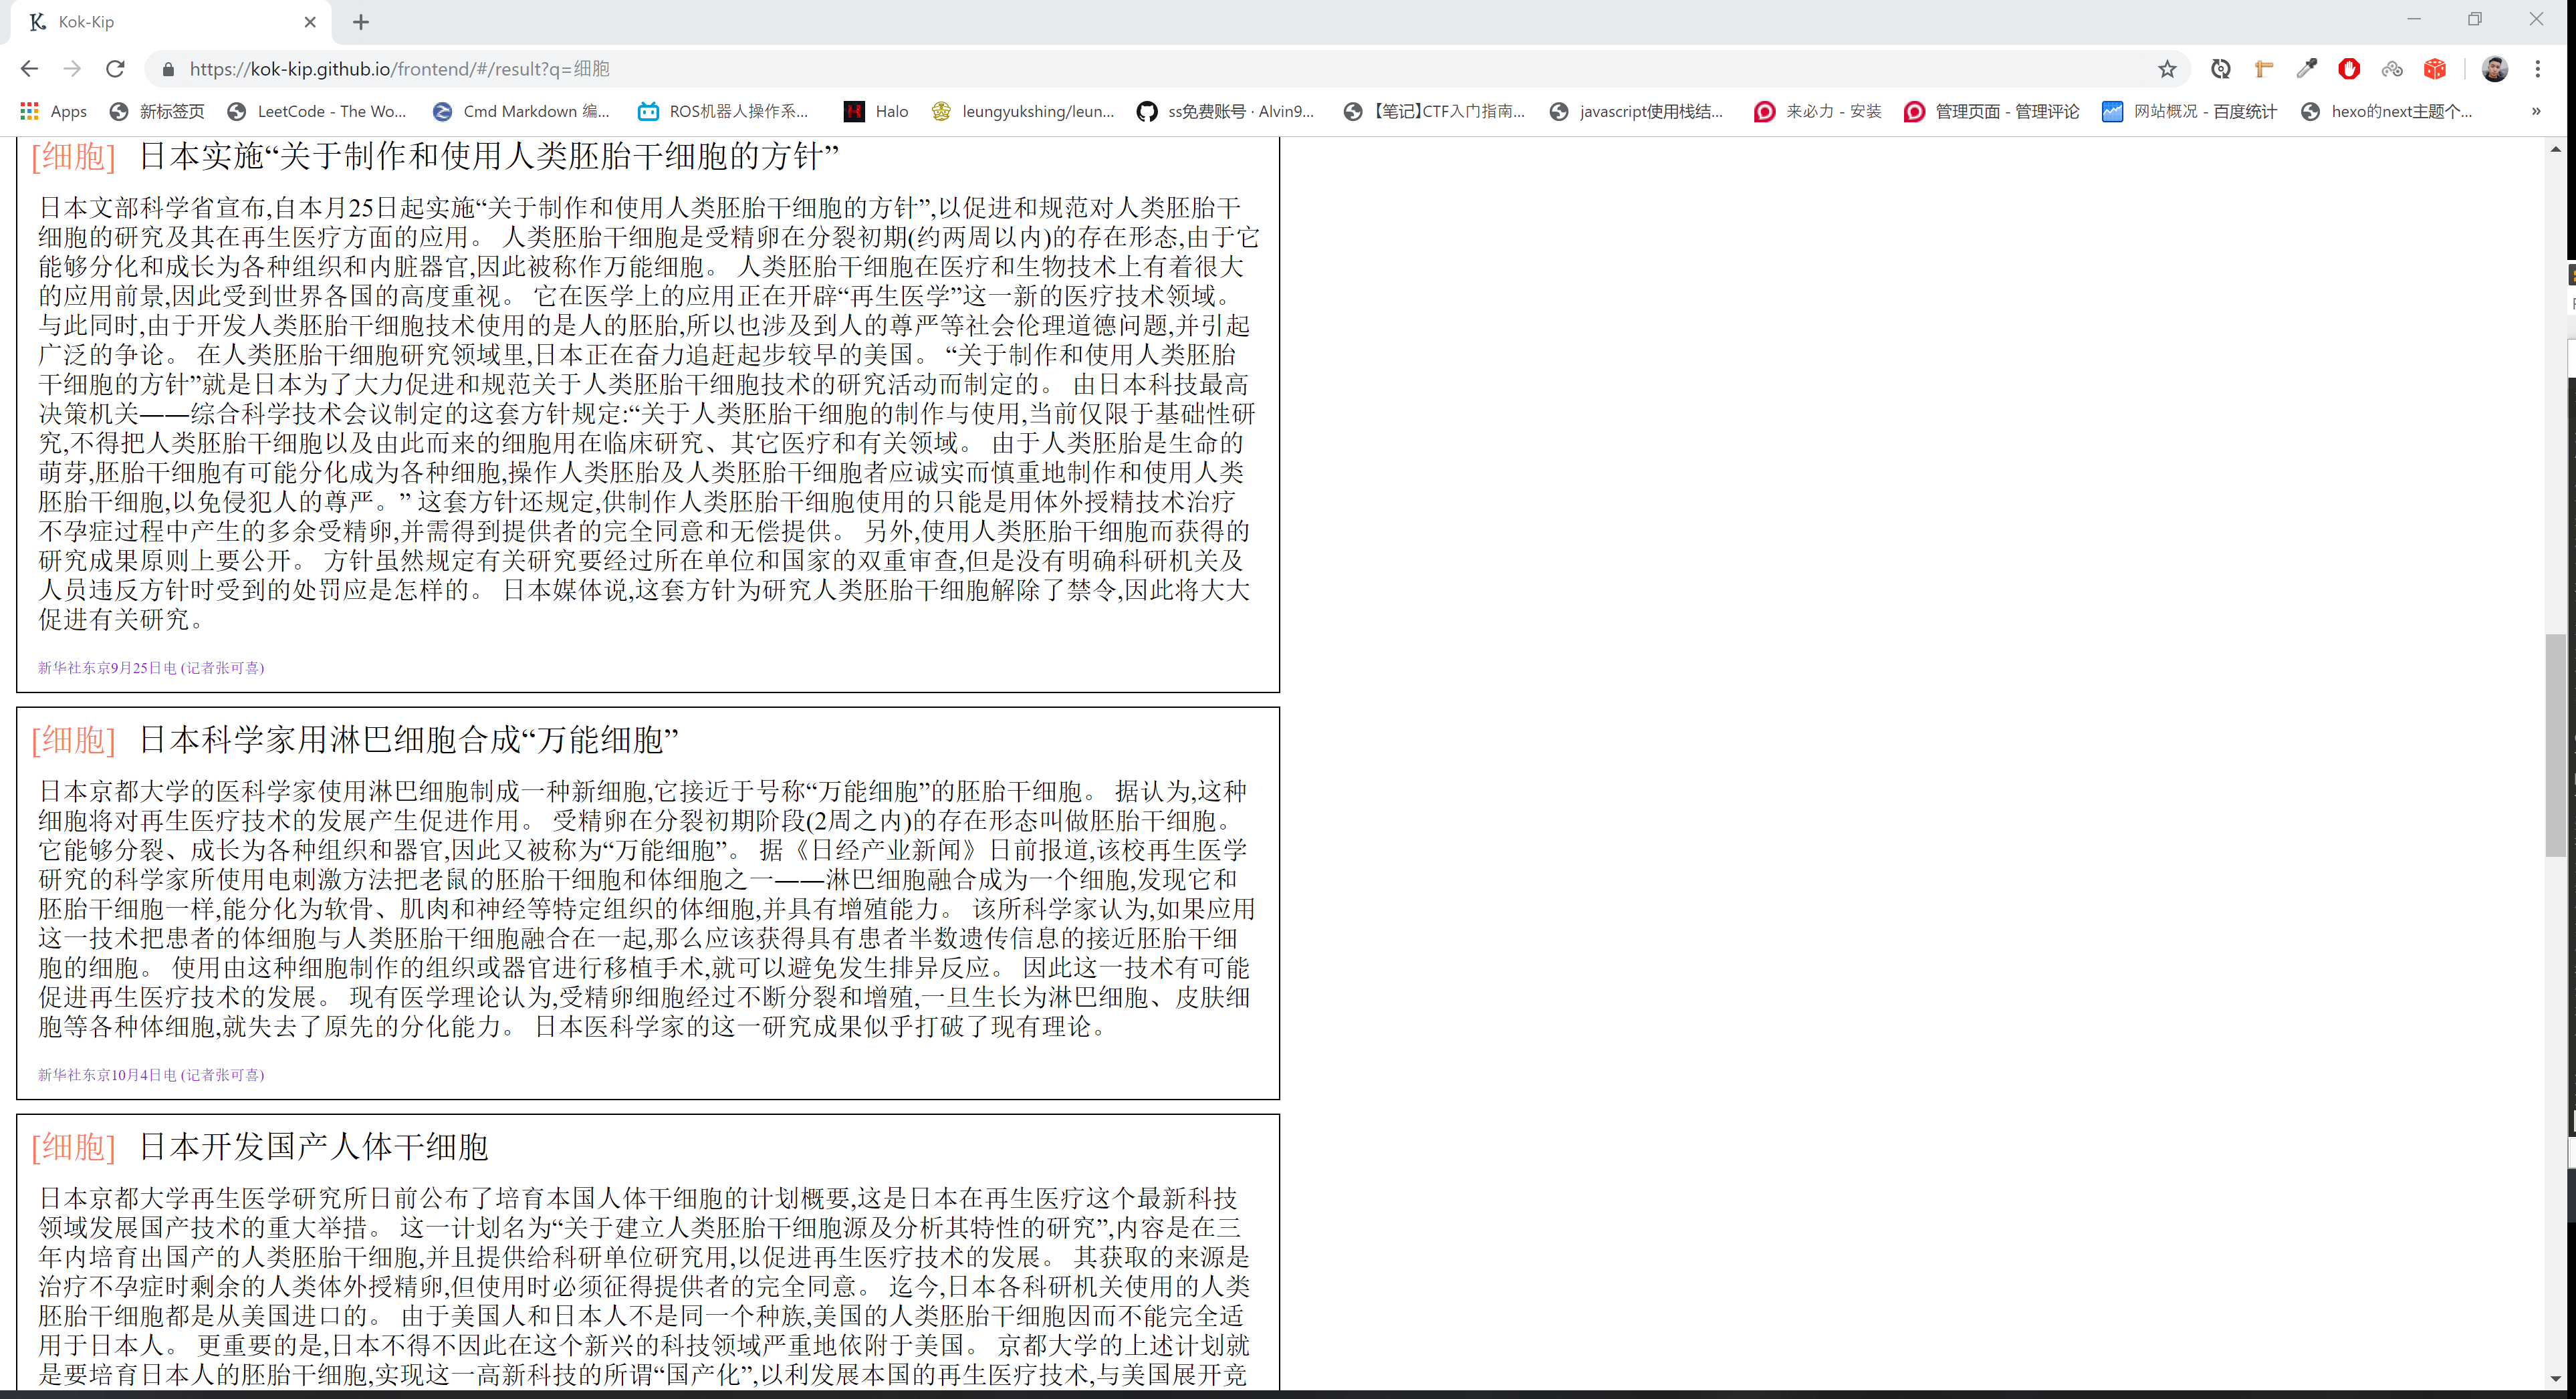
\includegraphics[width=3in]{./image/img5.png}
				\caption{Search Result for 细胞 3}
			\end{minipage}%
		}%
		\subfigure{
			\begin{minipage}[]{0.5\linewidth}
				\centering
				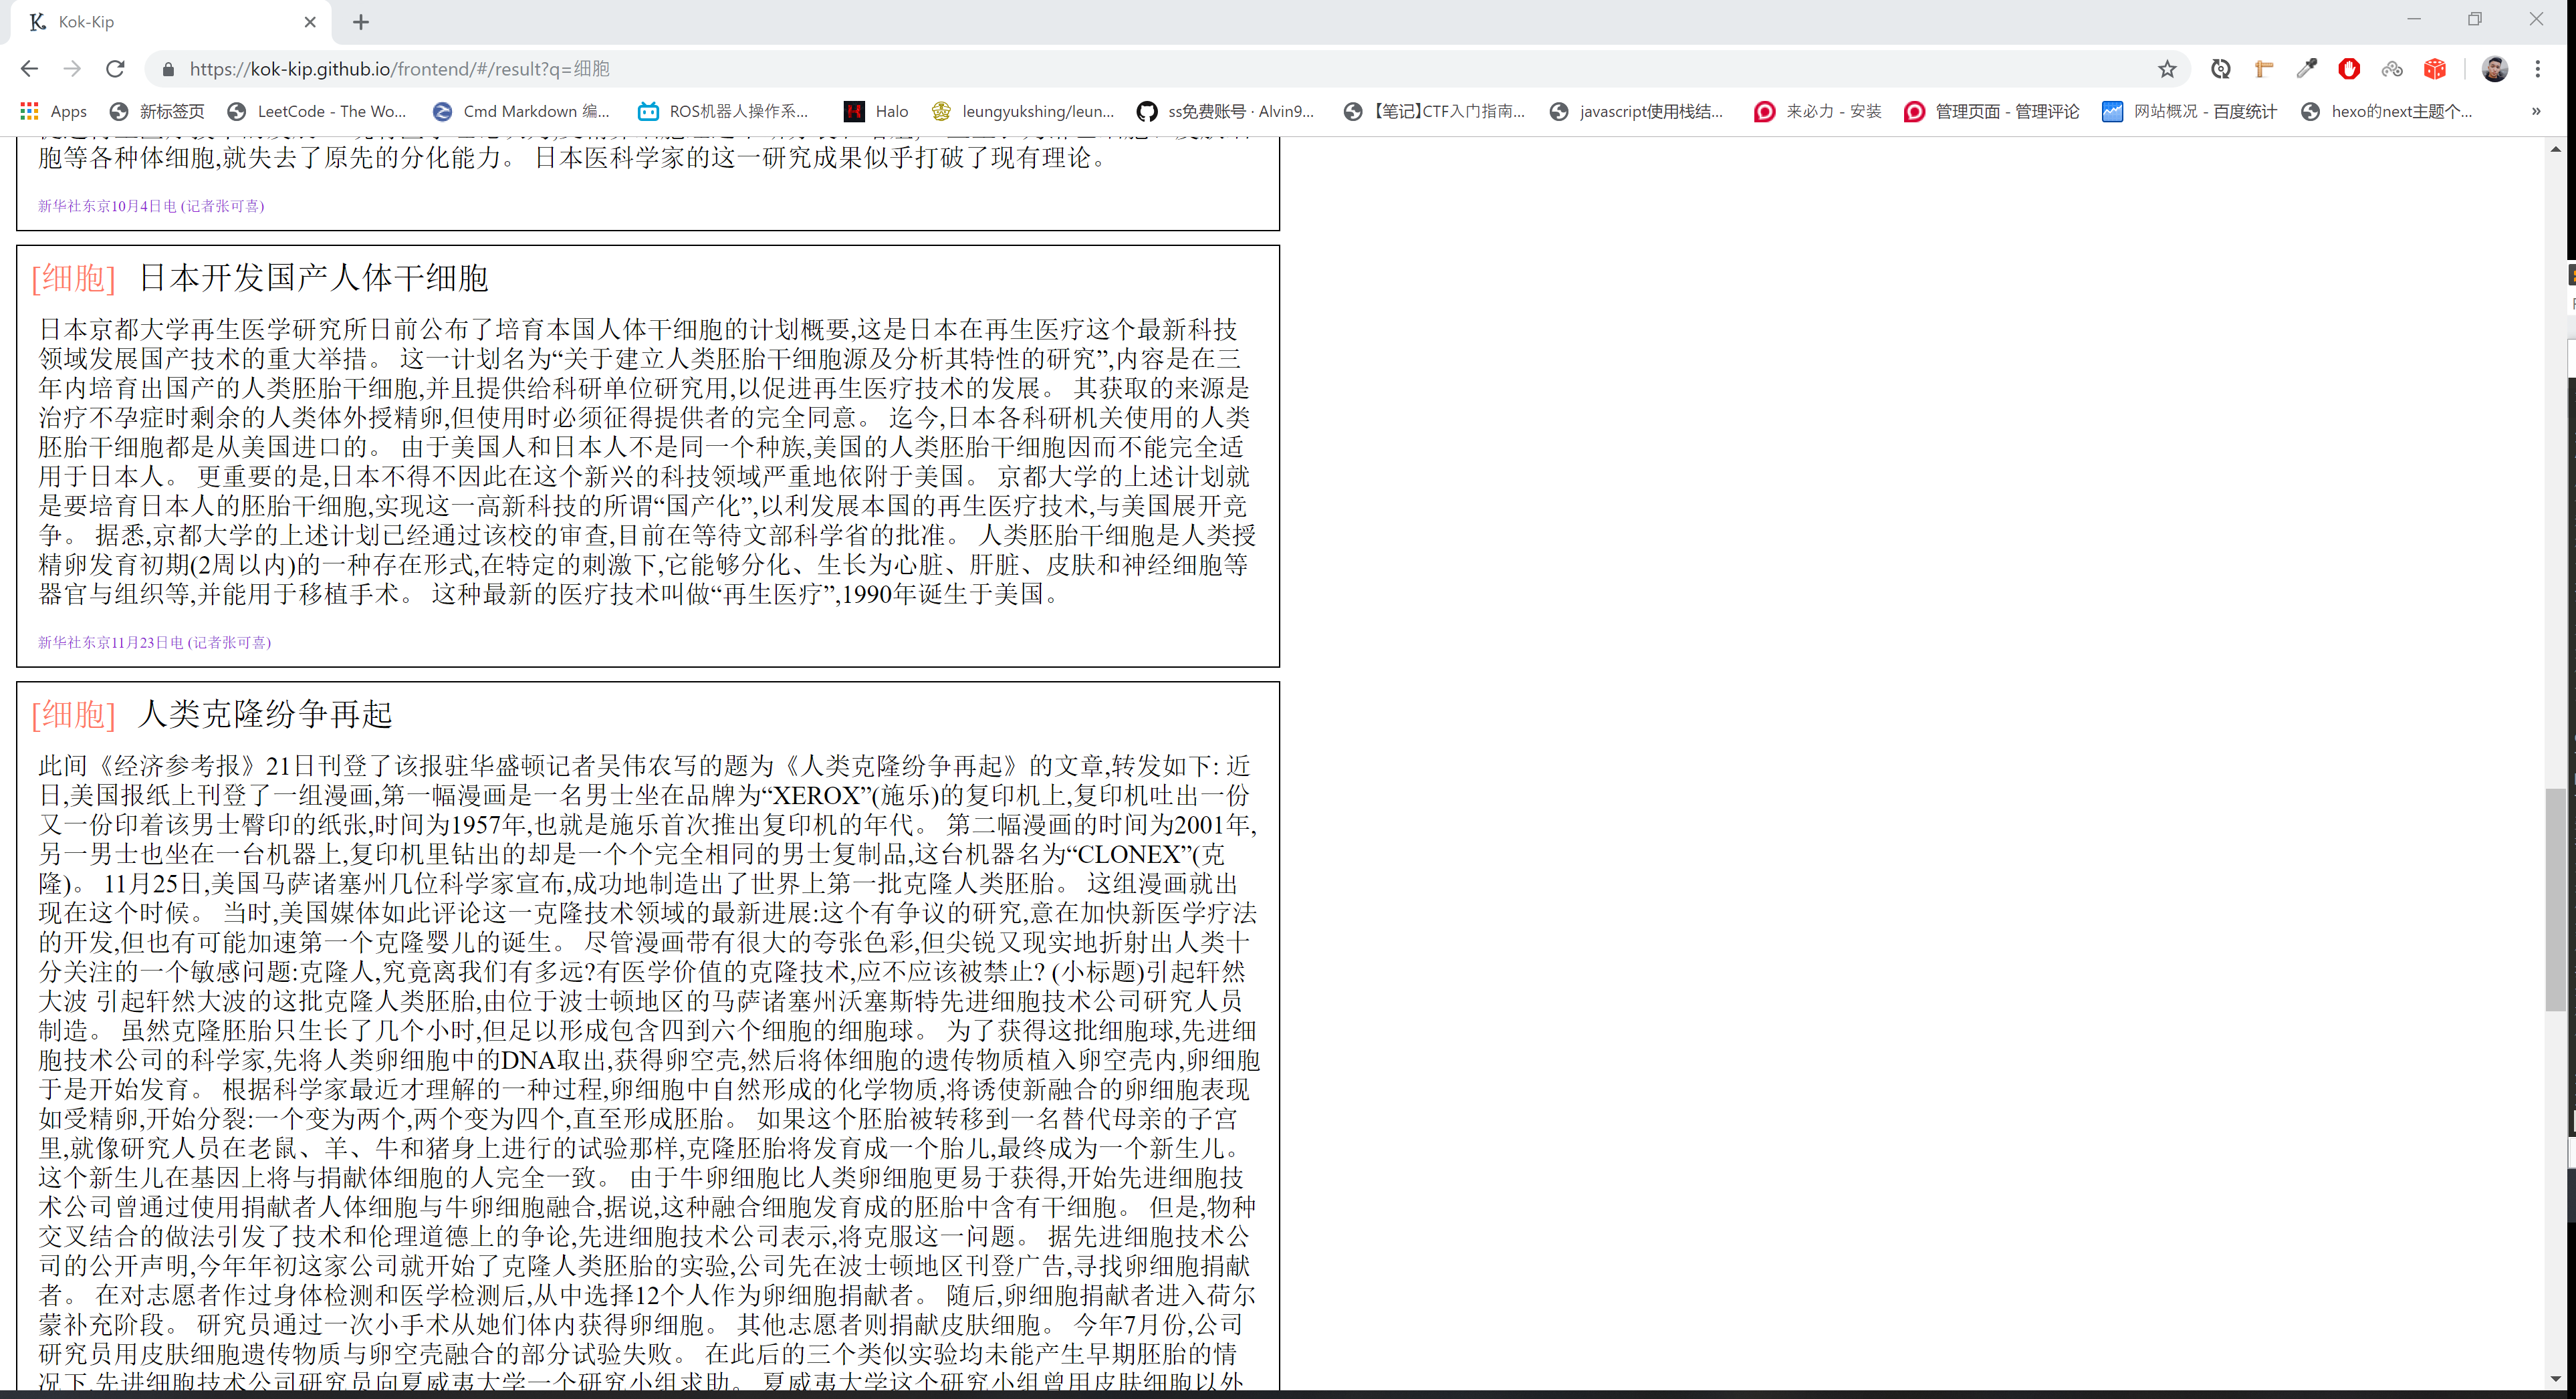
\includegraphics[width=3in]{./image/img6}
				\caption{Search Result for 细胞 4}
			\end{minipage}%
		}%
		\centering
	\end{figure}
	Pay attention to the second picture, We can see the 4th document does not exactly contain the query word, but its content, mostly relevant to clone technology, is greatly related to the query word. That what embedding could bring to us!
	
	% Part 4.2.2: Query 2
	\subsubsection{Query Word: 中国}
	\begin{figure}[H]
		\centering
		\subfigure{
			\begin{minipage}[]{0.5\linewidth}
				\centering
				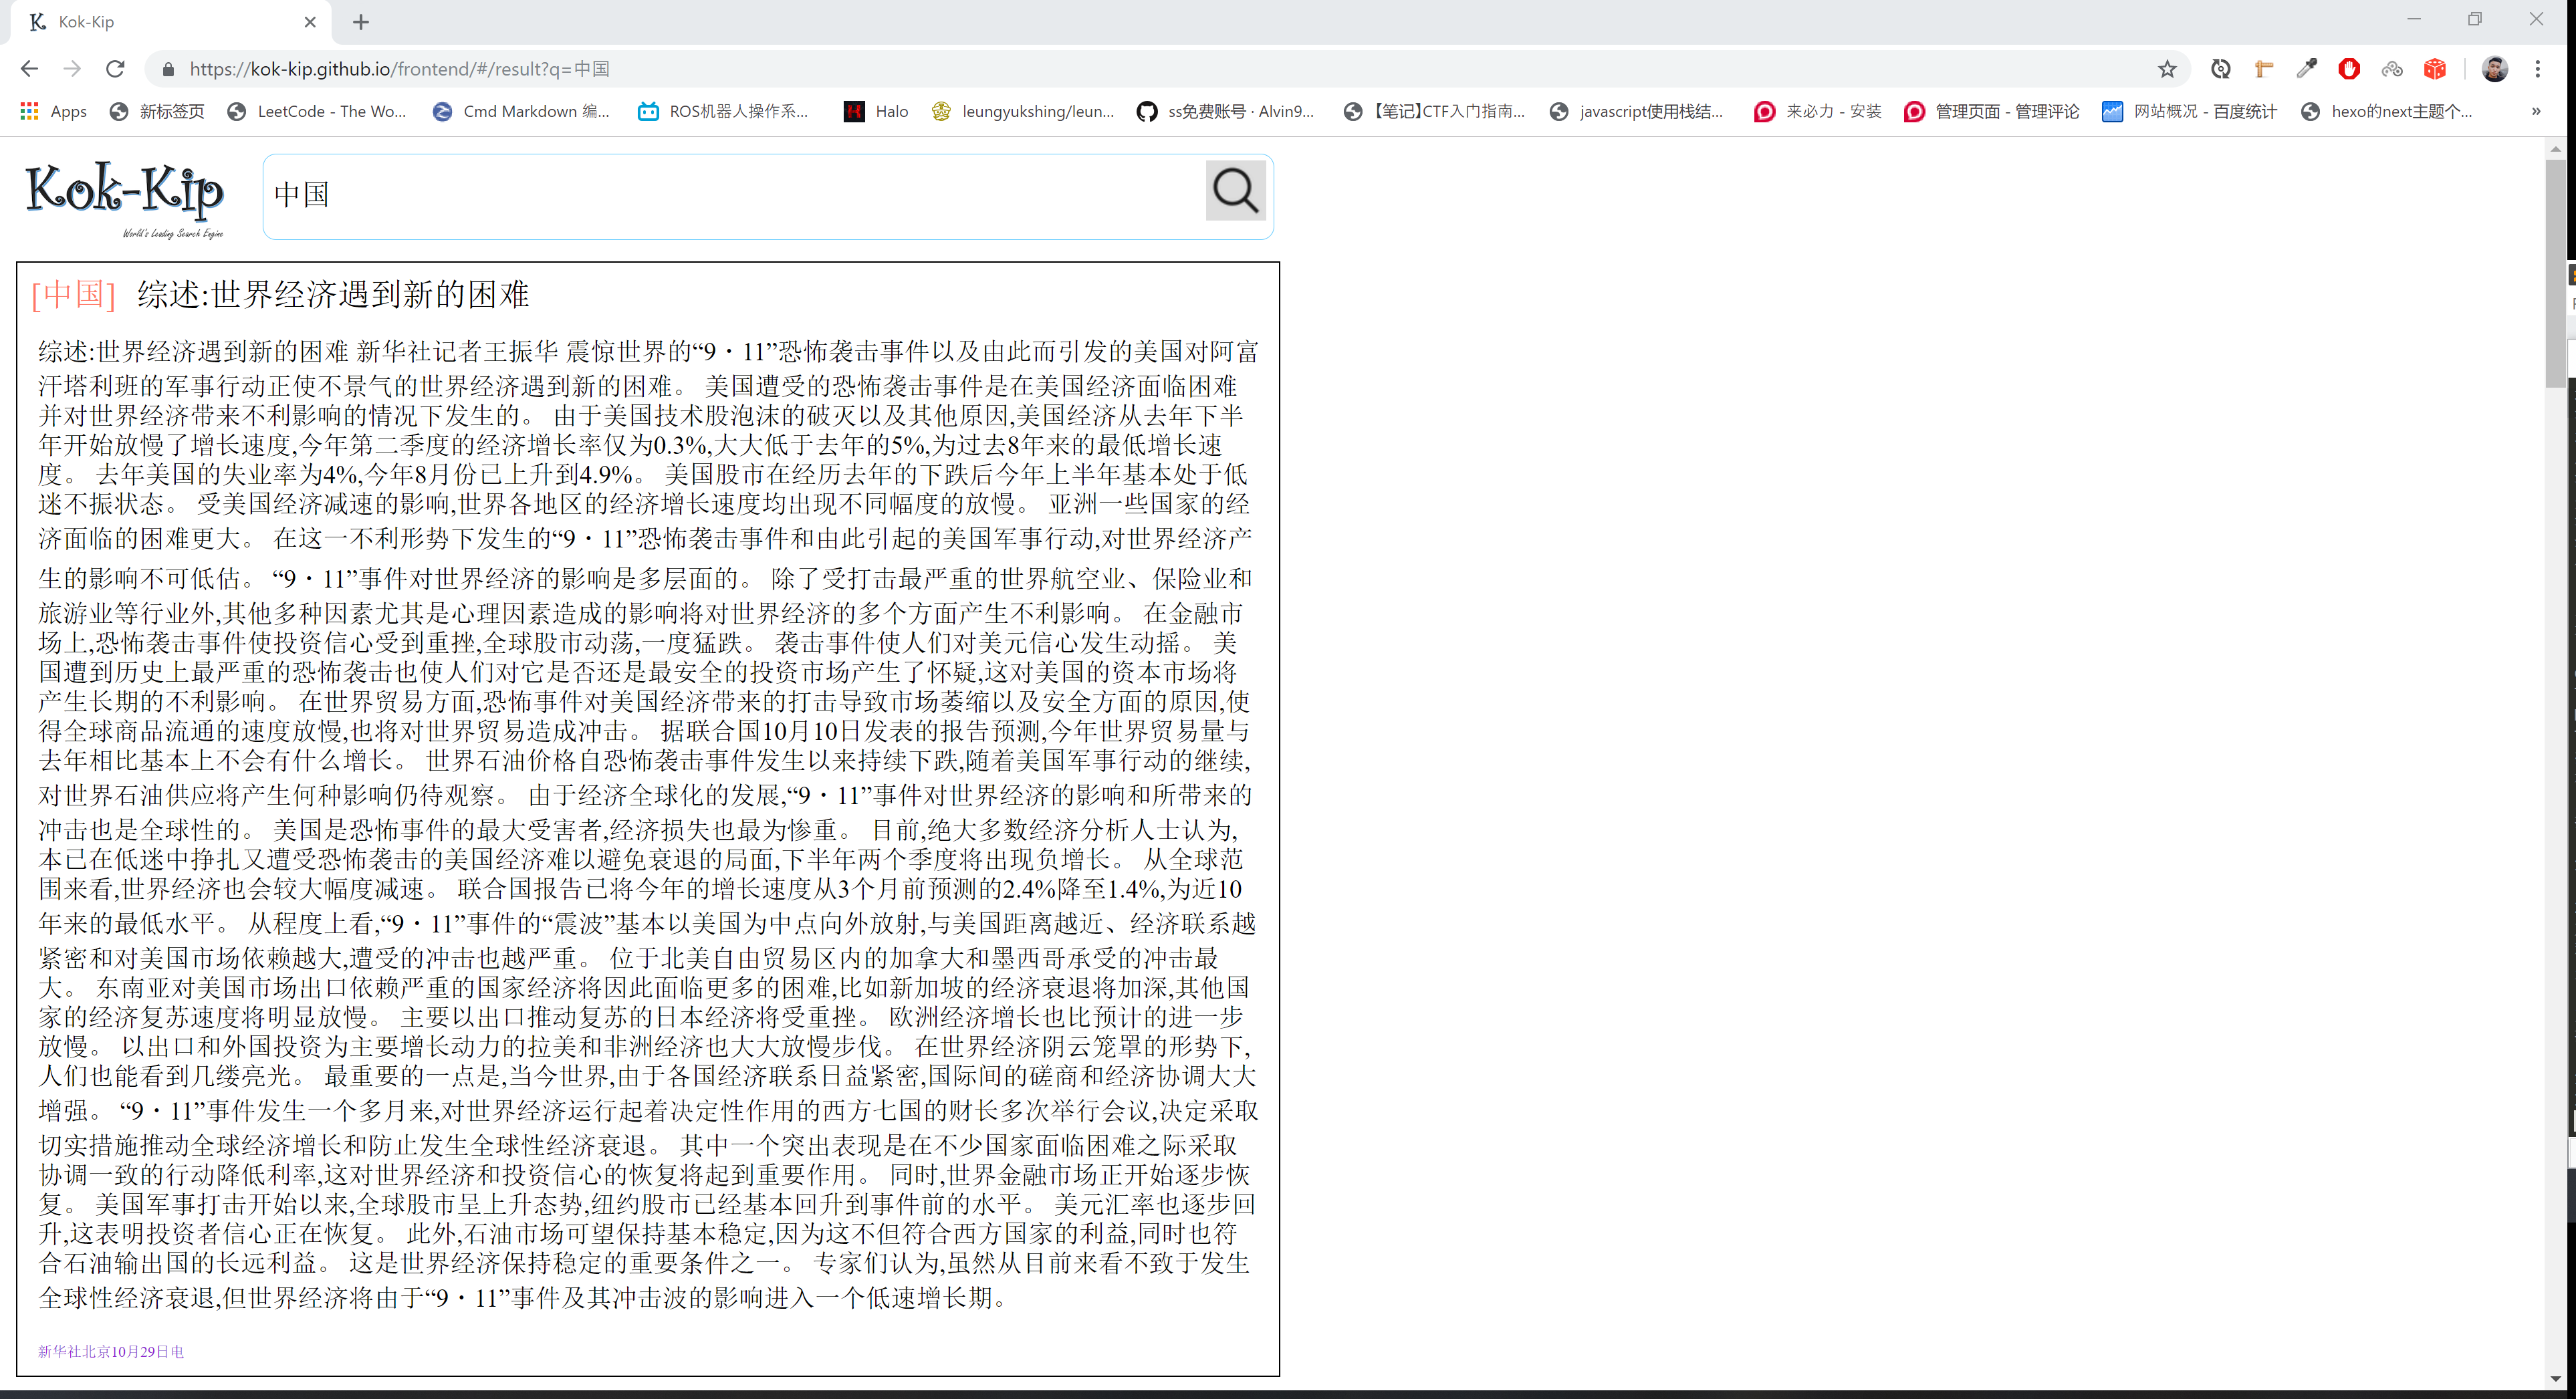
\includegraphics[width=3in]{./image/img7}
				\caption{Search Result for 中国 1}
			\end{minipage}%
		}%
		\subfigure{
			\begin{minipage}[]{0.5\linewidth}
				\centering
				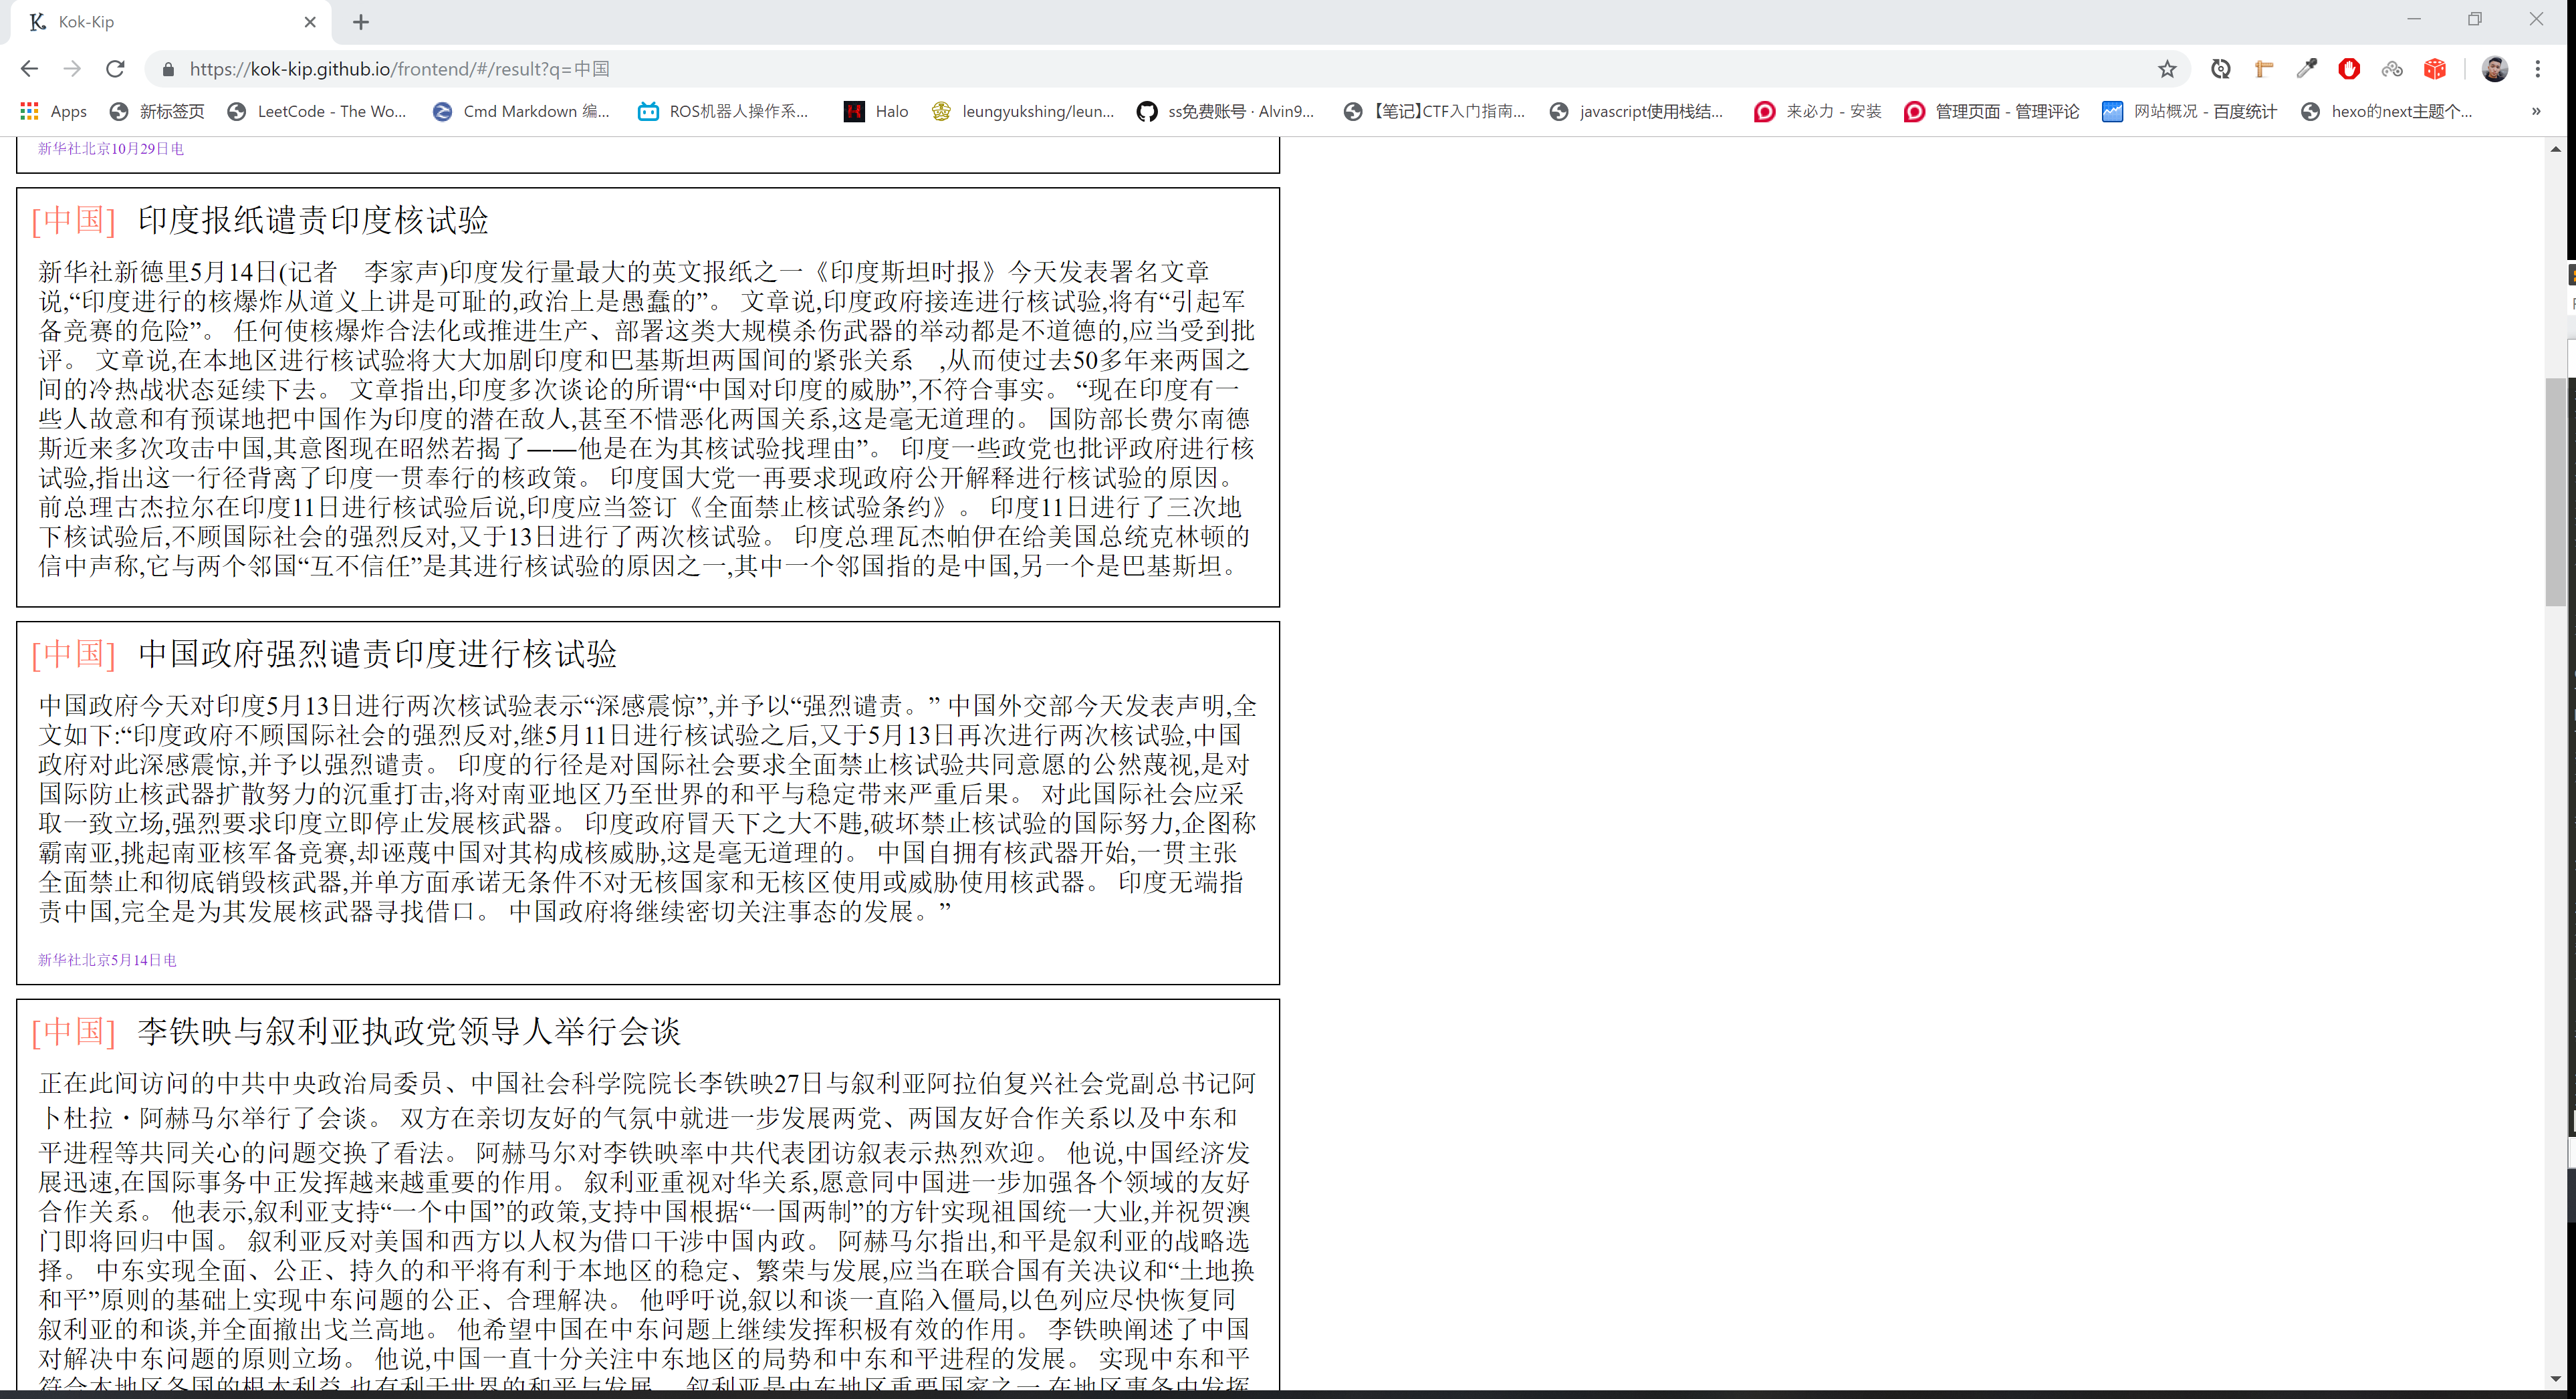
\includegraphics[width=3in]{./image/img8}
				\caption{Search Result for 中国 2}
			\end{minipage}%
		}%
		\centering
	\end{figure}
	
	\begin{figure}[H]
		\centering
		\subfigure{
			\begin{minipage}[]{0.5\linewidth}
				\centering
				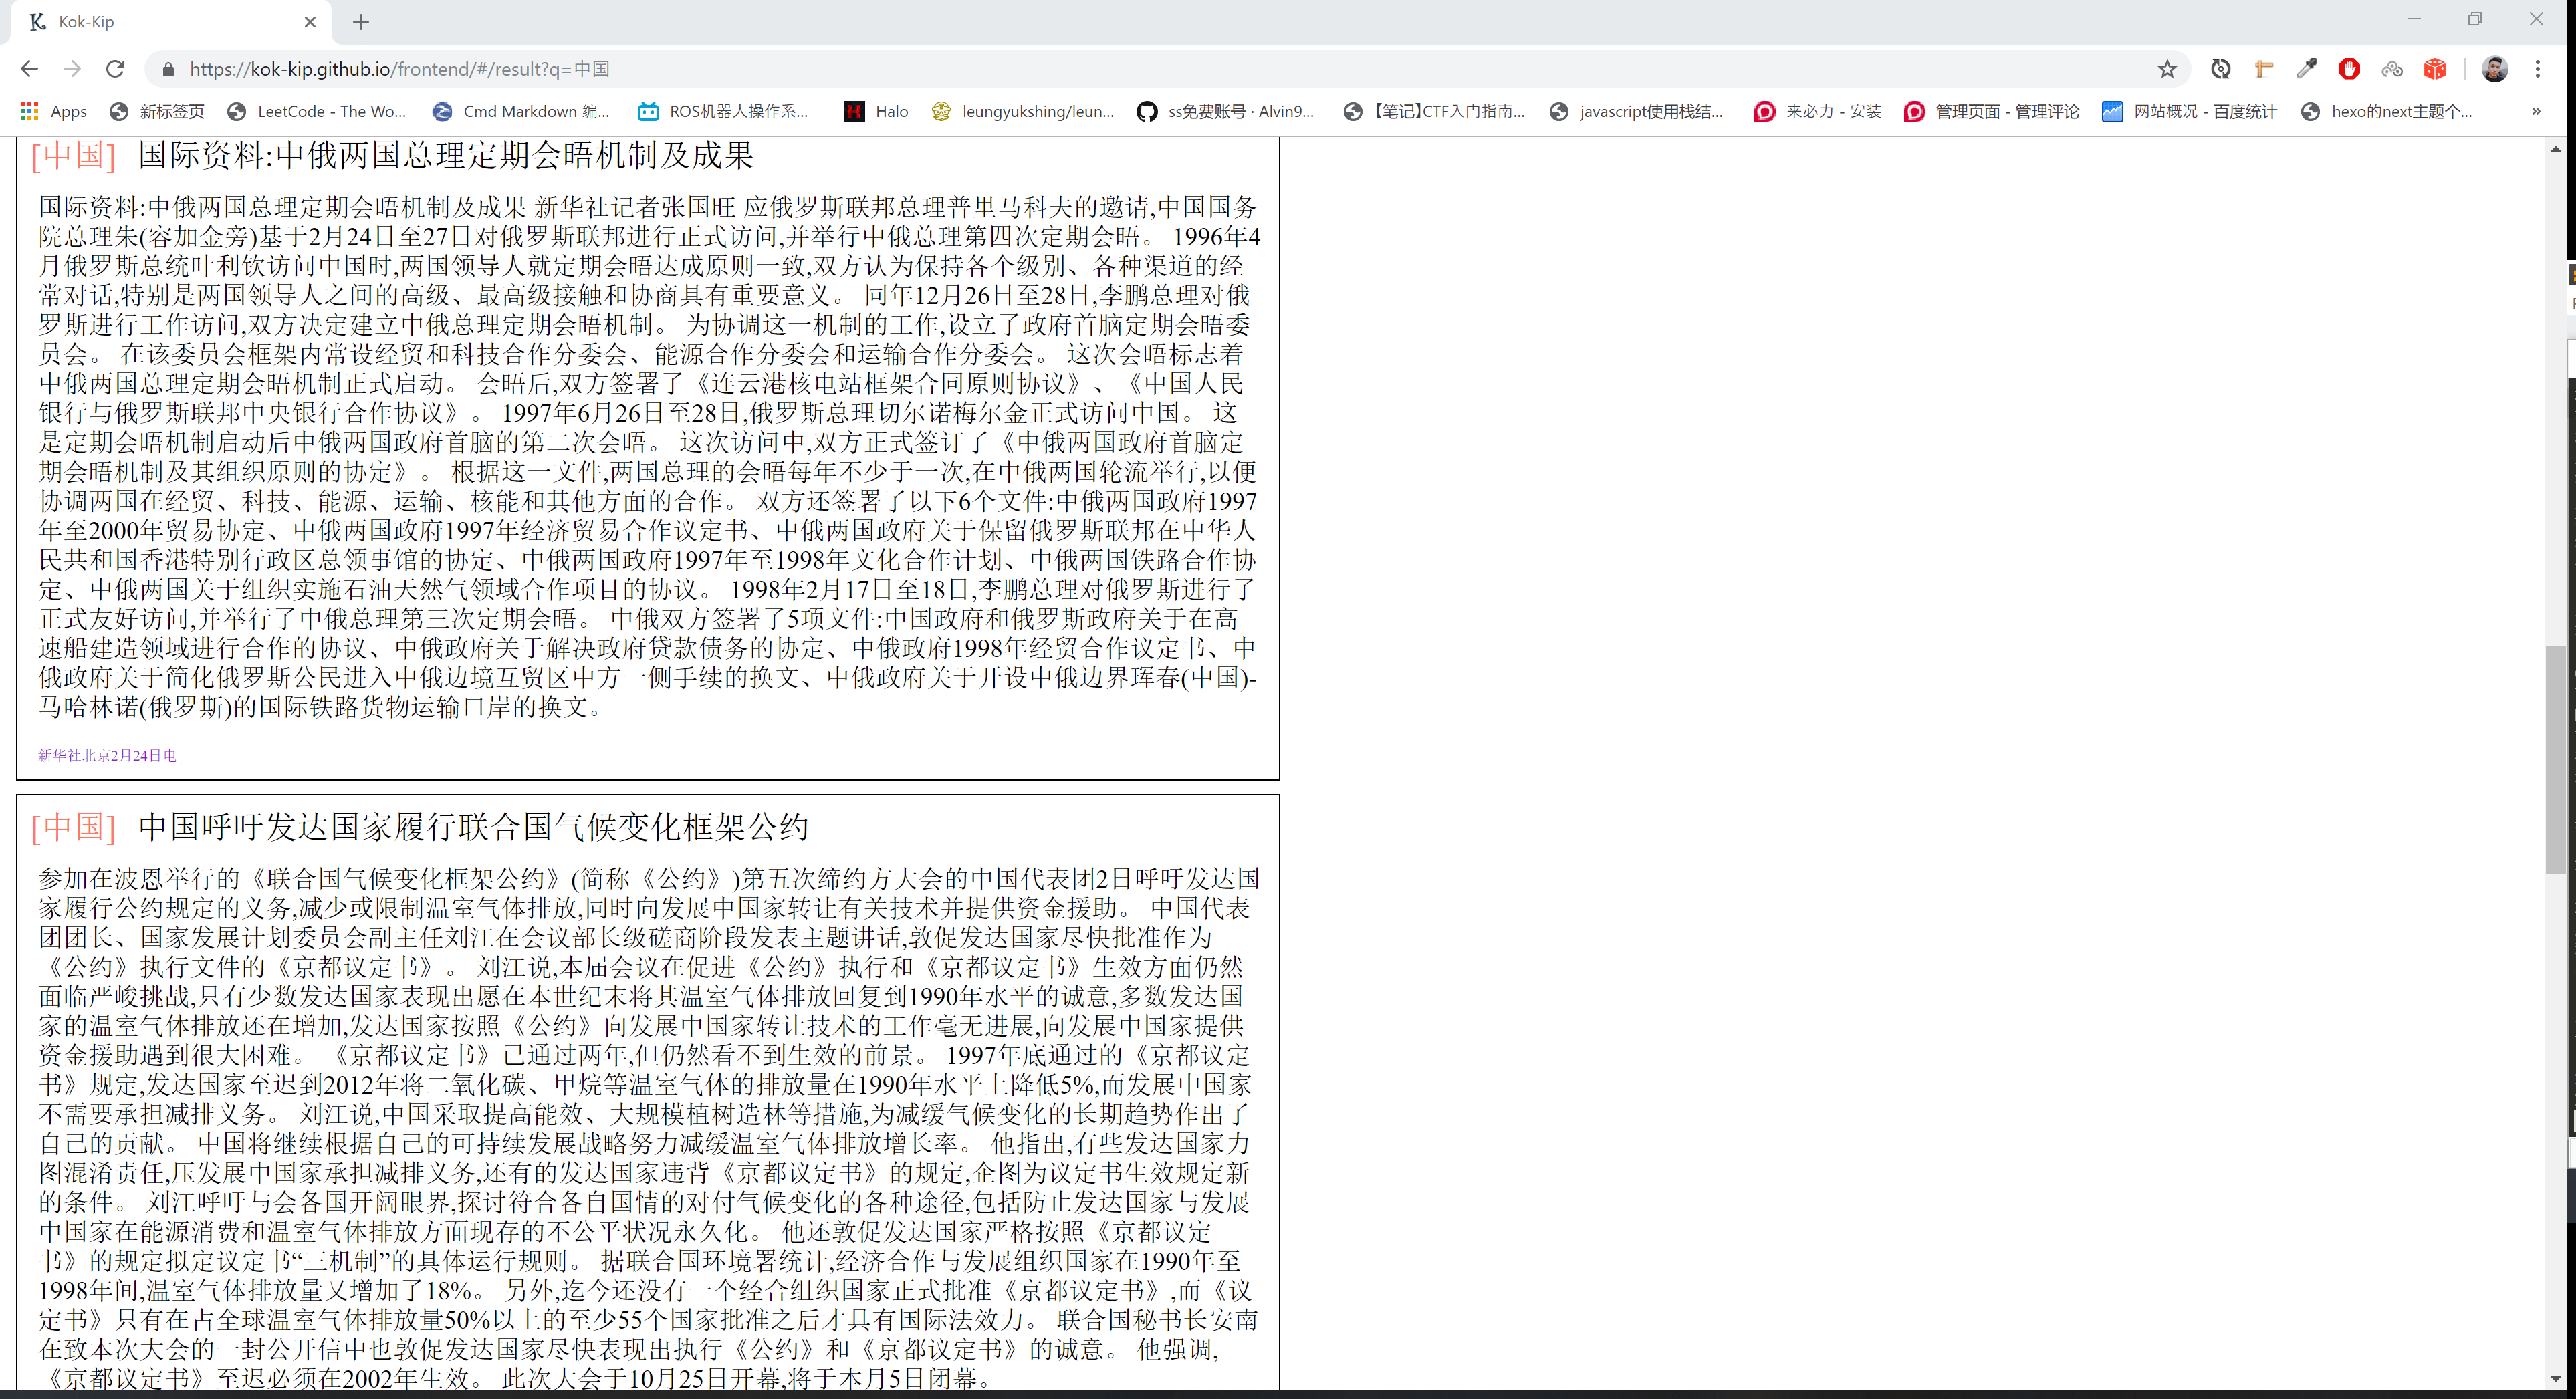
\includegraphics[width=3in]{./image/img9}
				\caption{Search Result for 中国 3}
			\end{minipage}%
		}%
		\subfigure{
			\begin{minipage}[]{0.5\linewidth}
				\centering
				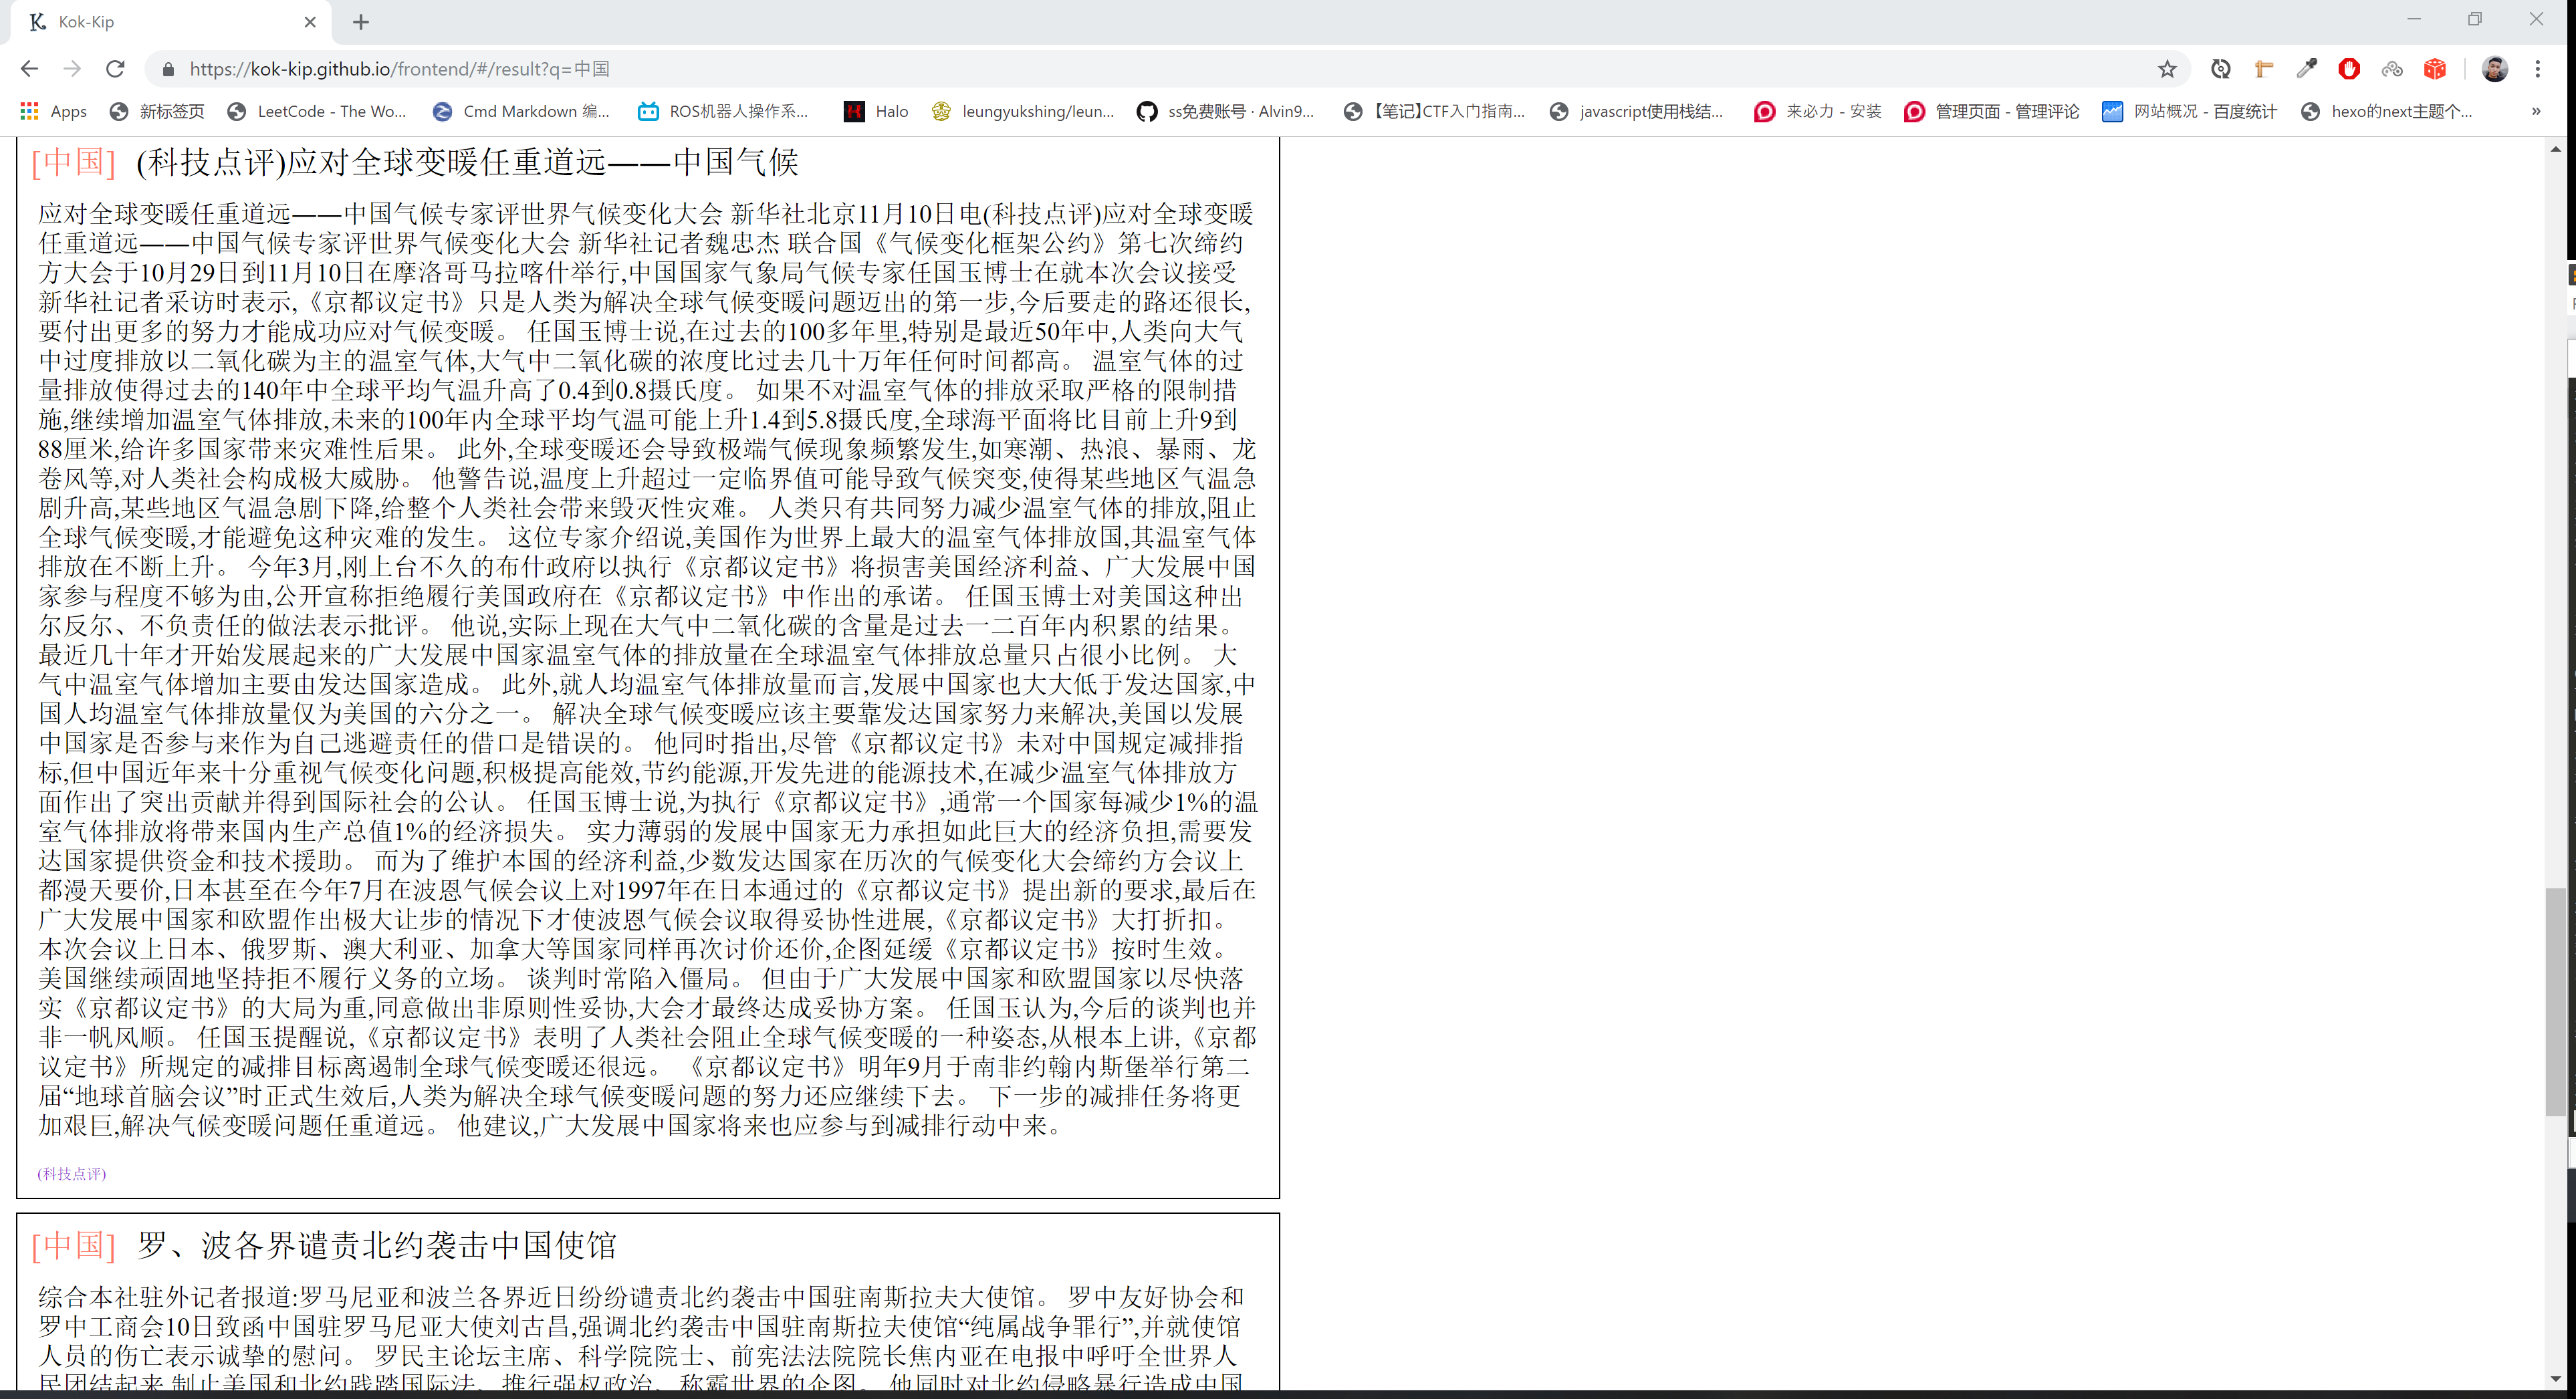
\includegraphics[width=3in]{./image/img10}
				\caption{Search Result for 中国 4}
			\end{minipage}%
		}%
		\centering
	\end{figure}
	From picture 2 again, we can see that the 2nd document talks about India, which is semanticly close to our query word, which proves our embedding technology works well.
	
	% Part 4.2.3: Query 3
	\subsubsection{Query Word: 气候}
	\begin{figure}[H]
		\centering
		\subfigure{
			\begin{minipage}[]{0.5\linewidth}
				\centering
				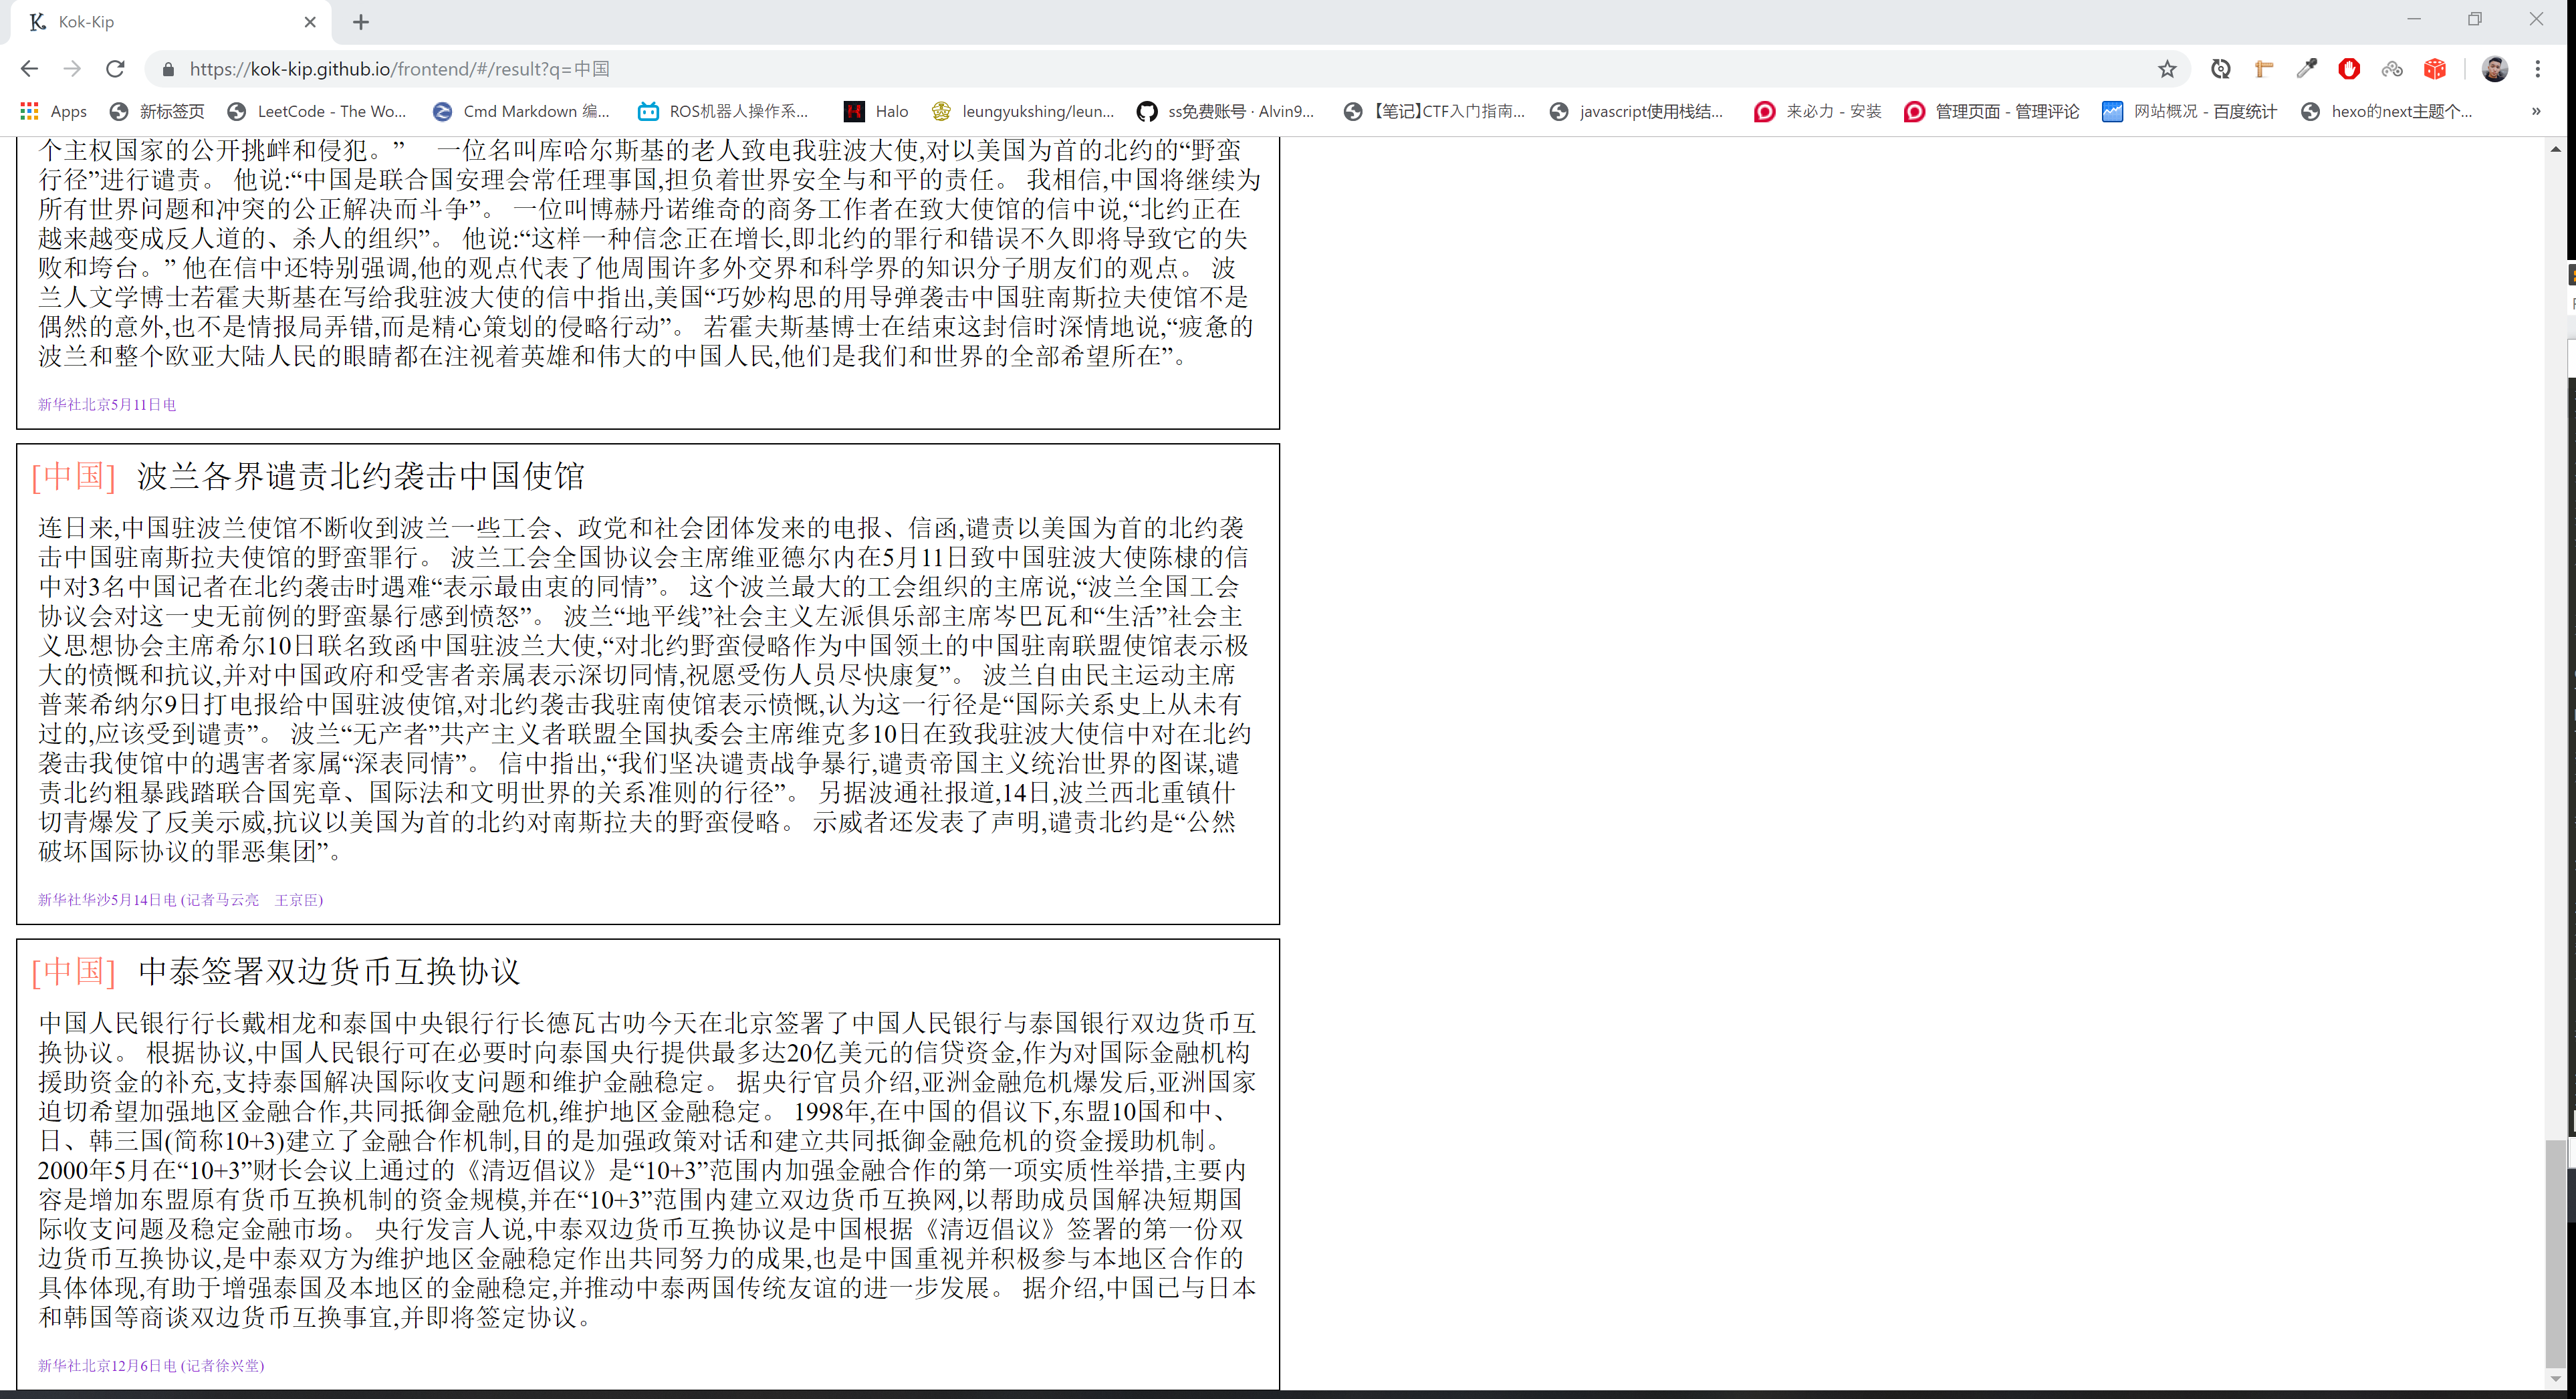
\includegraphics[width=3in]{./image/img11}
				\caption{Search Result for 气候 1}
			\end{minipage}%
		}%
		\subfigure{
			\begin{minipage}[]{0.5\linewidth}
				\centering
				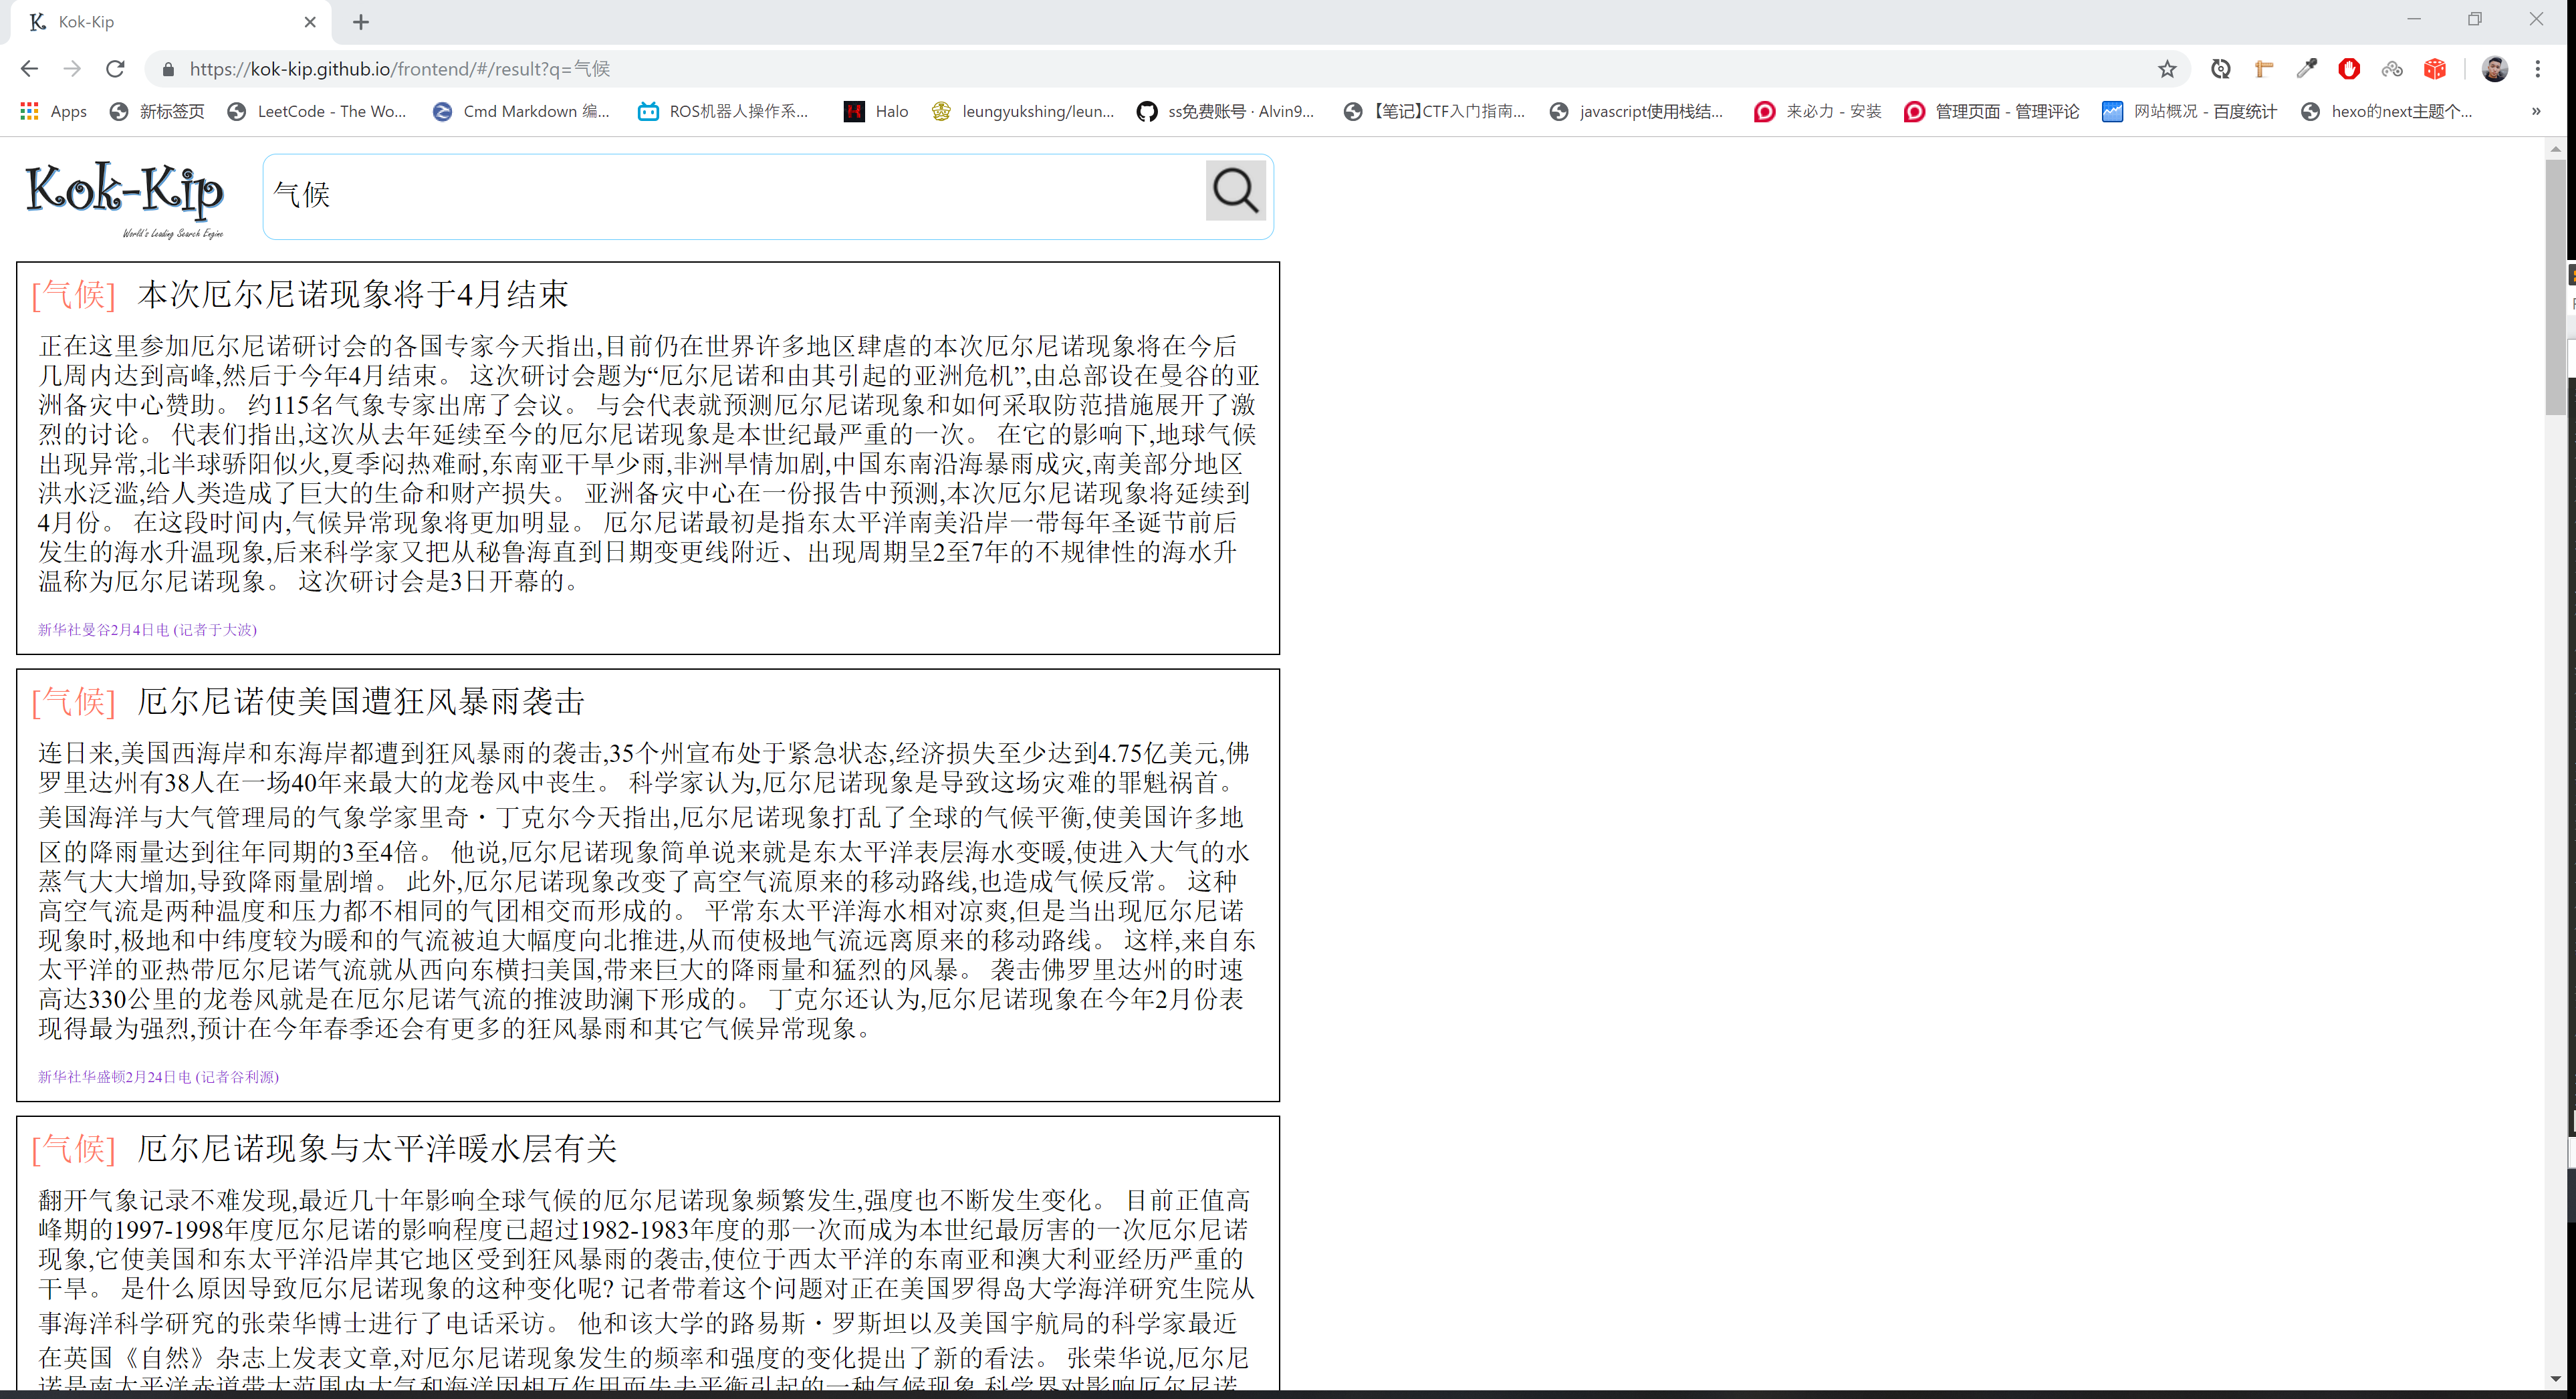
\includegraphics[width=3in]{./image/img12}
				\caption{Search Result for 气候 2}
			\end{minipage}%
		}%
		\centering
	\end{figure}
	
	\begin{figure}[H]
		\centering
		\subfigure{
			\begin{minipage}[]{0.5\linewidth}
				\centering
				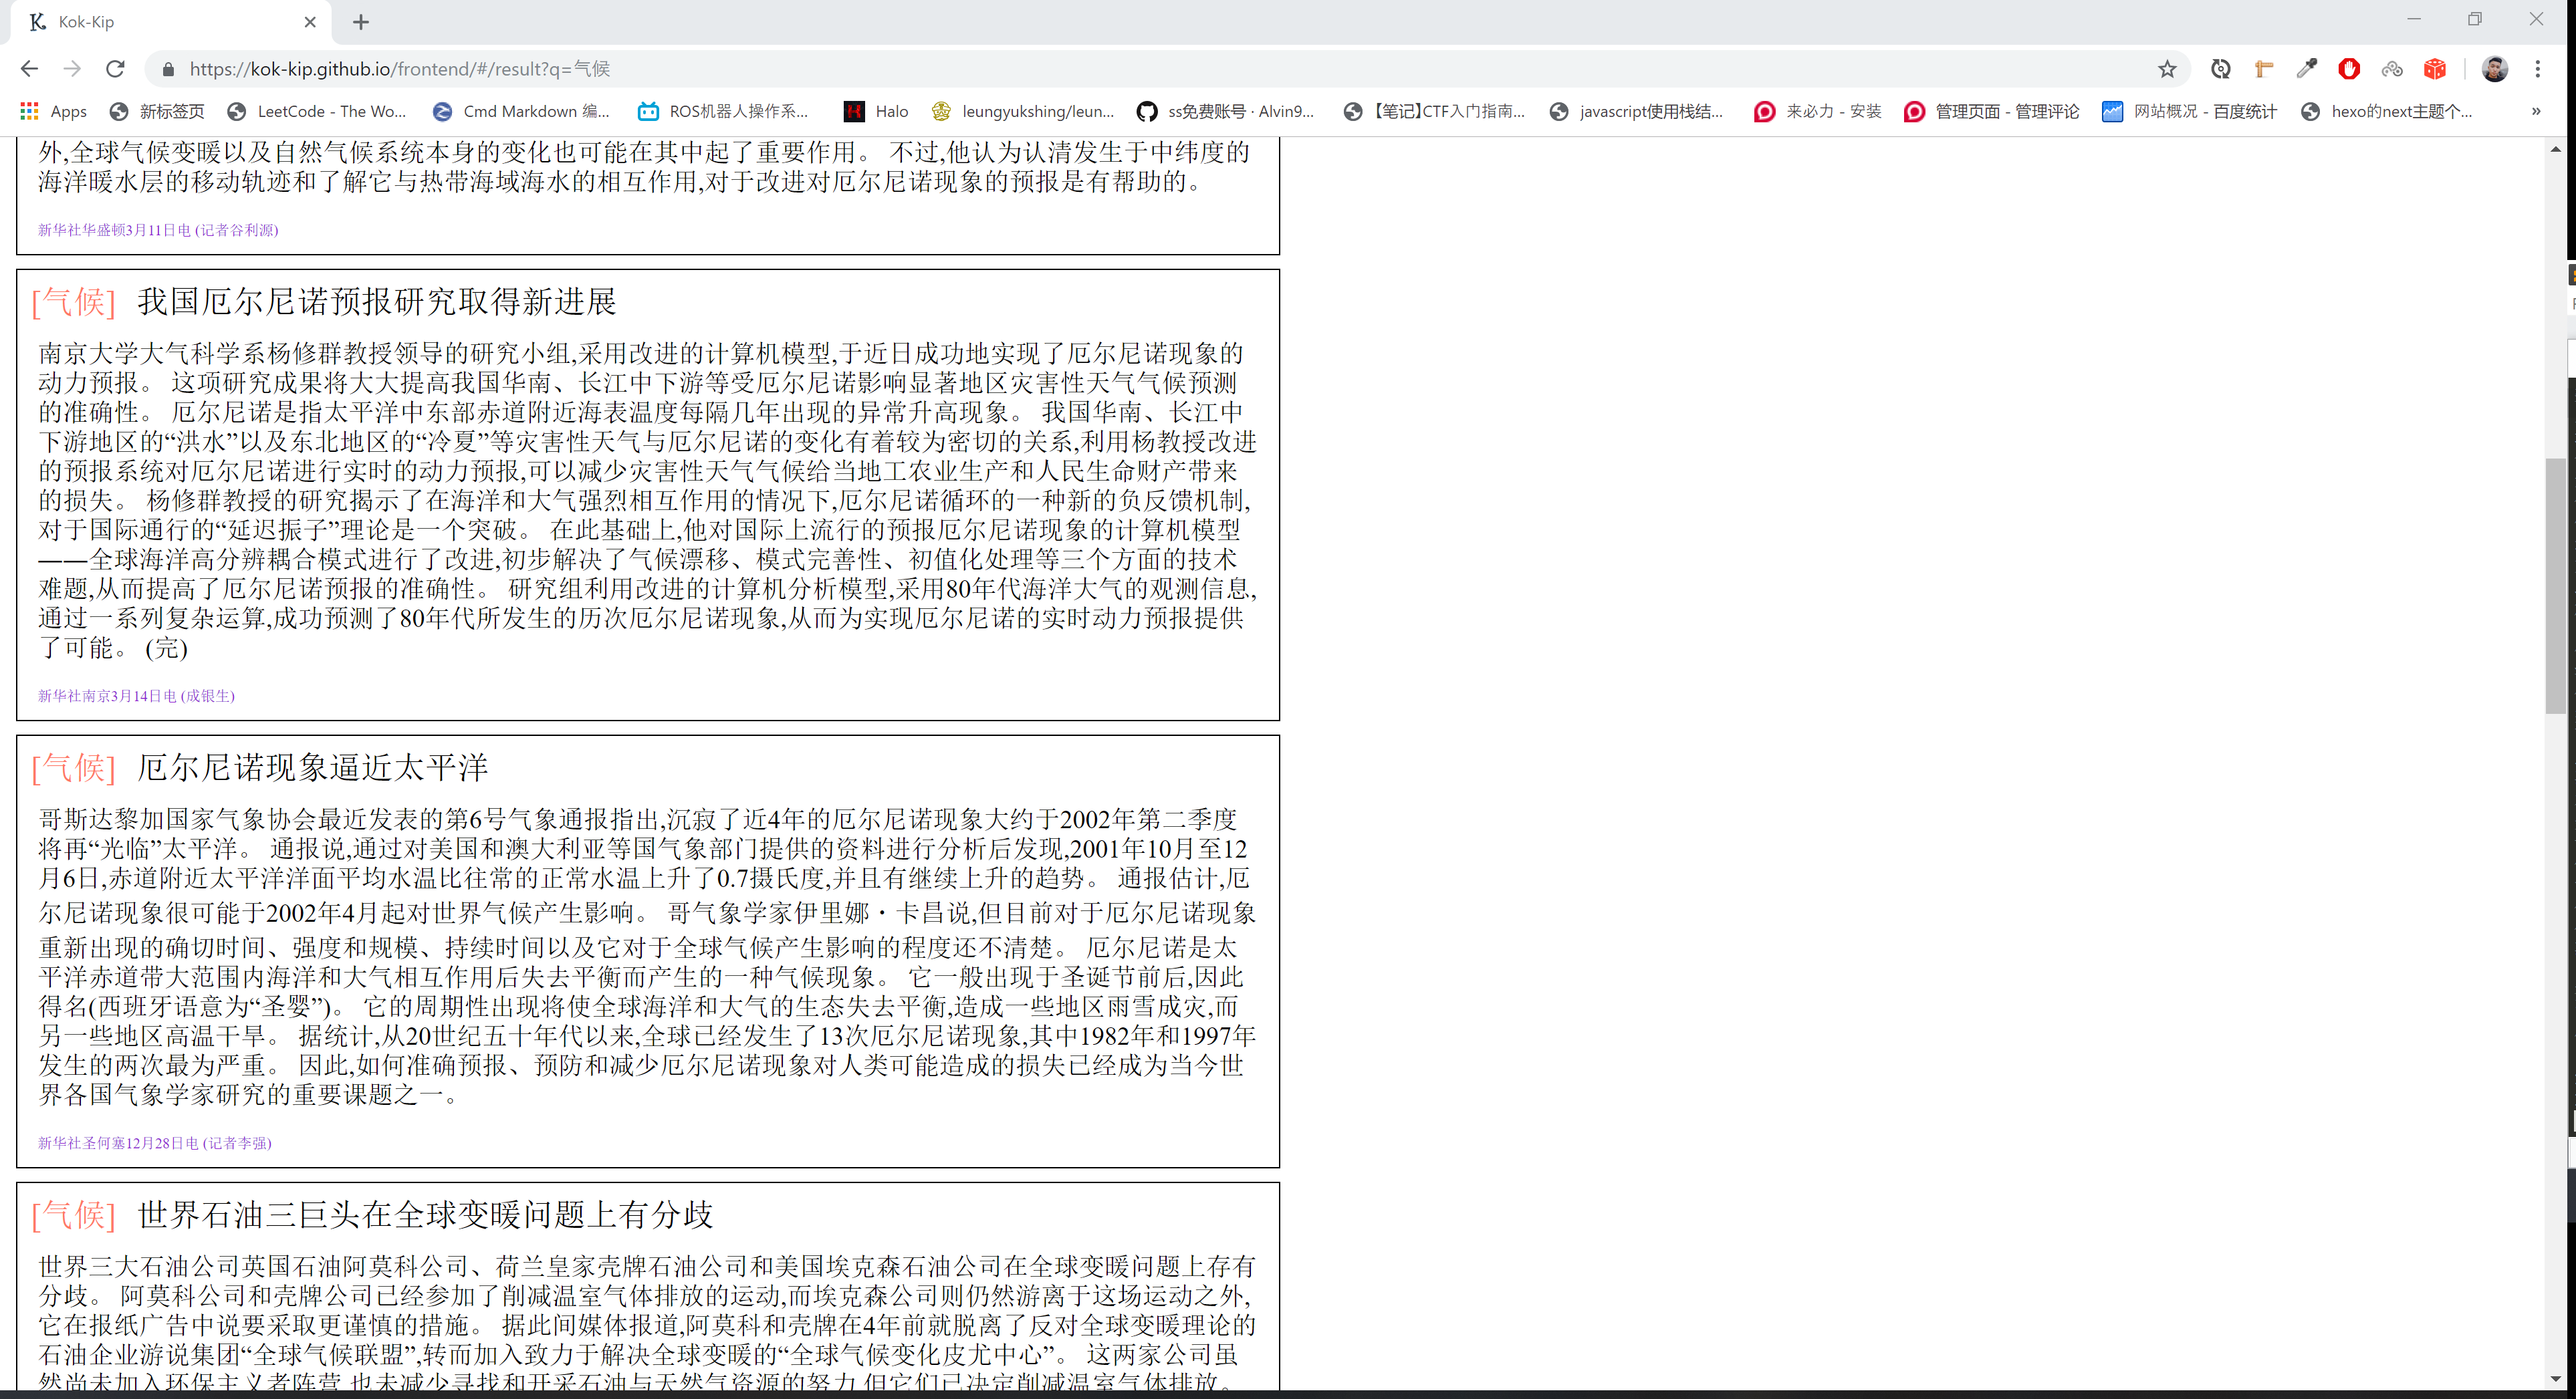
\includegraphics[width=3in]{./image/img13}
				\caption{Search Result for 气候 3}
			\end{minipage}%
		}%
		\subfigure{
			\begin{minipage}[]{0.5\linewidth}
				\centering
				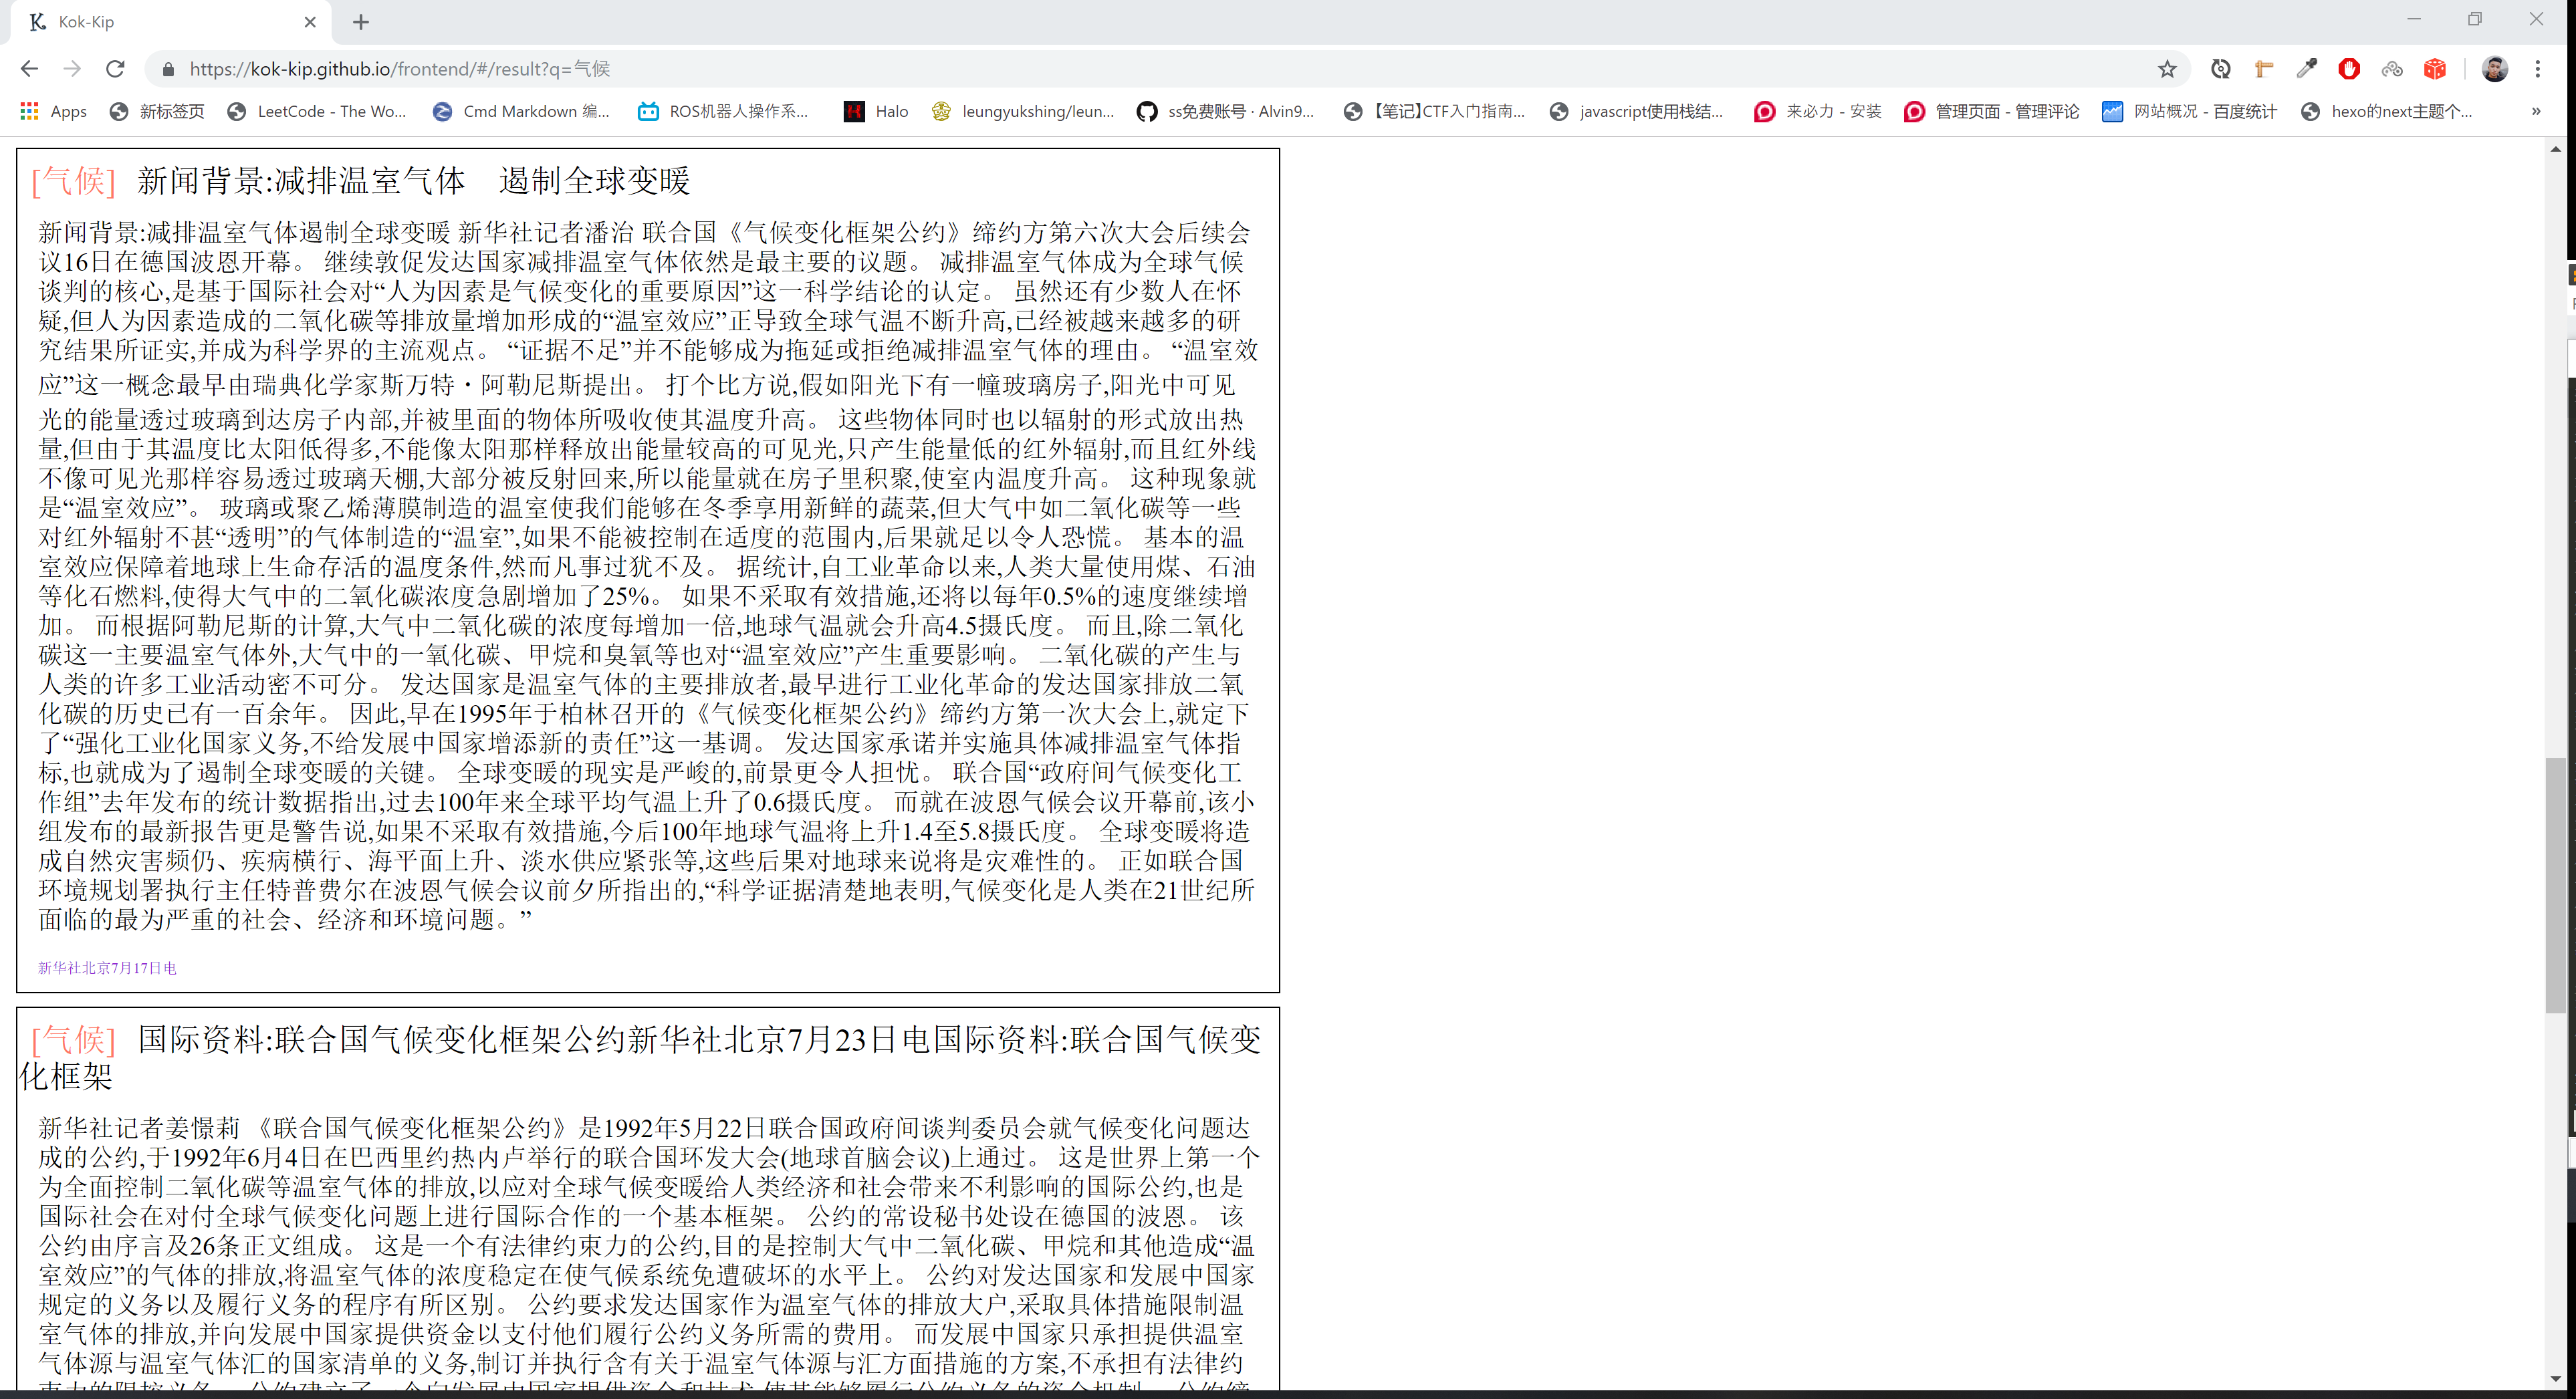
\includegraphics[width=3in]{./image/img14}
				\caption{Search Result for 气候 4}
			\end{minipage}%
		}%
		\centering
	\end{figure}
	As you can see, all documents returned are very relevant to the query word.

	% Part 4.3 Latency Metrics
	\subsection{Latency Metrics}
	 End-to-end latency is an importance metrics for a search engine so we should also report our latency. We obtain latency data from server log. The average e2e latency is about 8 seconds. TFIDF costs 0.15 seconds, and BM25 costs 0.02 seconds, while Word Embedding costs approximately 2 seconds. The rest of latency is used for document parsing.
   Given the fact that we do not use index in our database and we just run this server on a laptops, a 2 seconds latency in our calculation is definitely acceptable. What we can optimize is that we could store the documents in database so that we do not need to parse them every time, which could reduce latency drastically.
	
	% Part 5 Future Work
	\section{Future Work}
	Our engine is largely limited by the embedding model. We can access the Tencent Corpus Dataset, but it is unlikely to load it into a word2Vec model due to its large size. Thus what we neet to do is that we should filter those high frequency words from the dataset and load them into a model, which could improve search accuracy greatly.
	Also, our dataset size is too small to support a popular document searching. We may support incremental documents and thus enlarge our document pool to return more relevant results.And it would be better to store the files in database instead of parsing them every time. Of course constructing index would benefit query efficiency.
	Morover, we may try to extract information from documents if they share a similar content structure. This may provide more significant information regarding themselves.
	Last, we are going to deploy this service in a remote server so we may have more computational resource. But it will take some time to find a suitable machine.
	
	% Part 6 Summary
	\section{Summary}
	Given limited time and resources, it's quite amazing for our team to finish this project. From design to implementation, we all do it by our own, without any reference. The most thing we want to present in this project is what we learn from Information Retrieval Course in this semester. Benefitting from Scrum, we assure our product's quality and have a clear division and cooperation. As depicted above, our search engine achieves good performance in this dataset and we believe it could perform well in other dataset.
	From this project, we have a deeper understanding of document retrieval, especially those relevant score algorithms. There is still a clear gap between an excellent search engine and what we have achieved. And we will perfect this project in the future.

	% Part 7 Acknowledge
	\section{Acknowledge}
	Sincerely thanks for Professor Shangsong Liang's supervision and suggestion during our development process.
	
	% Part 8 Division
	\section{Division}
	Yucheng Liang: Project Leader, is mainly responsible for project management, product design and backend development, as well as report writing. 

	Junhua Liang: Developer, is mainly responsible for frontend design, development, testing, report formatting as well.
	
	Guangtao Zeng: Developer, is mainly responsible for backend development, report writing as well.
	
	\bibliographystyle{unsrt}  
	%\bibliography{references}  %%% Remove comment to use the external .bib file (using bibtex).
	%%% and comment out the ``thebibliography'' section.
	%%% Comment out this section when you \bibliography{references} is enabled.
	\begin{thebibliography}{1}
		
		\bibitem{Web Search Engine}
		Sergey Brin, Lawrence Page.
		\newblock The Anatomy of a Large-Scale Hypertextual Web Search Engine.
		\newblock {\em Computer Science Department, Stanford University}.
		
		\bibitem{The Google PageRank Algorithm}
		\newblock The PageRank Citation Ranking:
		Bringing Order to the Web
		
		
		\bibitem{SimSeerX: A Similar Document Search Engine}
		Kyle Williams, Jian Wu, C.Lee Giles
		\newblock SimSeerX: A Similar Document Search Engine
		\newblock {\em The Pennsylvania State University, University Park}.
		
		\bibitem{A Full-Text-Based Search Engine for Finding Highly Matched Documents Across Multiple Categories}
		Hung D. Nguyen and Gynelle C. Steele.
		\newblock A Full-Text-Based Search Engine for Finding Highly Matched Documents Across Multiple Categories.
		\newblock {\em Glenn Research Center, Cleveland, Ohio}.
		
		\bibitem{A Semantic Search Engine for Indexing and Retrieval of Relavent Text Documents}
		Jayalakshmi T S, C Chethana.
		\newblock A Semantic Search Engine for Indexing and Retrieval of Relavent Text Documents.
		\newblock {\em PES College of Engg}.	
		
		\bibitem{Distributed Representations of Words and Phrases and their Compositionality}
		Tomas Mikolov, Ilya Sutskever, Kai Chen, Greg Corrado, Jeffrey Dean.
		\newblock Distributed Representations of Words and Phrases and their Compositionality.
		\newblock {\em Google Inc. Mountain View}.
		
		
		
	\end{thebibliography}
	
\end{document}
